% MSc Dissertation - A Visual Trace Map of Edinburgh Place Names in Literature
% Merritt Wang | Supervisor: Uta Hinrichs | University of Edinburgh | 2026
 
\documentclass[logo,msc]{infthesis}
\usepackage{msccheck}
\usepackage{graphicx}
\usepackage{subcaption}
\usepackage{float}
\usepackage{longtable}
\usepackage{tabularx}
\usepackage{wasysym}
\usepackage{tikz}
\usepackage{pdfpages}
\usepackage{microtype}
\usepackage[hidelinks]{hyperref}
\usepackage{booktabs}
\usepackage{xcolor}
\usepackage{array}
\usepackage{enumitem}
 
\begin{document}
\begin{preliminary}
 
\title{A Visual Trace Map of Edinburgh Place Names in Literature}
\author{Merritt Wang}
\date{\today}
 
\abstract{
Existing digital tools for literary geography plot place names as points on a map, treating them as geographic data. The meaning a place name carries in a literary text, however, comes from its narrative context rather than its coordinates, and this dissertation asks whether that narrative structure can be made visible directly, using the LitLong Edinburgh database of 620 literary works (1687--2015), 2,135 place names, and 50,248 place-name mention records. Two research questions are addressed: RQ1 asks whether an author's distribution of place-name mentions across the city forms a visually distinctive spatial ``fingerprint,'' and RQ2 asks whether the co-occurrence of place names within literary works reveals a narrative topology distinct from their geographic topology. Six interactive D3.js visualisation prototypes were designed and implemented across these two directions: a radar chart, a bar-code fingerprint, and small-multiple maps for RQ1, and a force-directed network, a linear connection diagram, and a metro-style map for RQ2, all evaluated through a user study with domain-expert and general-public participants. The corpus analysis underlying RQ2 shows that Leith and Princes Street, roughly 2.5km apart, are the most strongly co-occurring place pair in the corpus (28 shared works). Rebuilding the metro-style map's line structure from measured co-occurrence rather than hand-drawn geography raises the proportion of adjacent stations sharing a real book from 22\% to 88\%, surfacing further instances of narrative structure that geographic proximity alone could not reveal. The user study ($n=13$) supports a qualified yes for RQ1: across all shape-to-author matching attempts, the radar chart reached 69\% accuracy against a 20\% chance baseline, with the bar-code and small-multiples designs close to half correct, and the radar chart the most consistently distinguishable design across every measure used, though single-shape identification accuracy was more modest and varied considerably by design.
}
 
\maketitle
 
\newenvironment{ethics}
   {\begin{frontenv}{Research Ethics Approval}{\LARGE}}
   {\end{frontenv}\newpage}
 
\begin{ethics}
This project obtained approval from the Informatics Research Ethics committee.\\
Ethics application number: 446635\\
Date when approval was obtained: 13 May 2026\\
The participants' information sheet and a consent form are included in the appendix.\\
\standarddeclaration
\end{ethics}
 
\begin{acknowledgements}
I would like to thank my supervisor, Uta Hinrichs, for her guidance and feedback throughout this project. I am also grateful to the School of Informatics at the University of Edinburgh for the resources and support that made this dissertation possible, and to everyone who took part in the user study.
\end{acknowledgements}
 
\tableofcontents
\listoffigures
 
\end{preliminary}
 
 
% ============================================================
% CHAPTER 1: INTRODUCTION
% ============================================================
\chapter{Introduction}
\label{chap:intro}

\section{Motivation}
 
Edinburgh has an unusually rich corpus of literary texts set in or concerning the city. The Palimpsest project at the University of Edinburgh systematically extracted place-name mentions from hundreds of these works spanning three centuries, producing the LitLong Edinburgh database: 620 documents published between 1687 and 2015, 2,135 distinct place names, and 50,248 geo-referenced mention records \cite{anderson2016}. The project made this corpus publicly accessible through a web interface that plots place mentions on an interactive geographic map.
 
Geographic maps are a natural starting point for literary data of this kind, but they carry an implicit assumption: that the meaning of a place name is determined by its location. That assumption holds up fine in geography, less so in literature. When Irvine Welsh names Leith in \textit{Trainspotting}, the word is not primarily a set of coordinates north of Edinburgh city centre; it evokes a social world, a class position, a political history. When Walter Scott names the Canongate, he is invoking a specific stratum of Edinburgh's past. A geographic map can show where these places are, but it has nothing to say about when in the narrative they appear, how often they recur, which other places surround them, or whose authorial voice chose them.

Place names in literary text, in other words, carry data about narrative structure as much as about geographic space. Accordingly, the visualisation problem tackled here is less about rendering literary geography more accurately on a map, and more about representing narrative structure in a form that reveals patterns geographic tools cannot.
 
\section{Problem Statement}
 
The core question this dissertation addresses is: can place names in literary text be visualised as an independent narrative structure, rather than as a rendering of geographic information?
 
It divides into two sub-problems corresponding to two distinct dimensions of narrative structure. The first concerns \emph{authorial spatial attention}: does each author's distribution of place-name mentions across Edinburgh constitute a distinctive pattern that can be recognised without prior knowledge of the author? The second concerns \emph{narrative co-occurrence}: do places that appear together across literary works form a topology that differs systematically from their geographic arrangement?
 
Existing tools do not address either question. They do not separate literary space from geographic space. They do not support comparison of authorial spatial styles. And they do not reveal which places are narratively proximate, as opposed to geographically proximate.
 
\section{Research Questions}
 
Two formal research questions guide the project:
 
\textbf{RQ1} (Author Spatial Fingerprint): Does each author's distribution of place-name mentions across Edinburgh's official neighbourhood sectors form a visually distinctive spatial signature, sufficient for users to identify authors from their fingerprint alone?
 
\textbf{RQ2} (Narrative Topology): Does the co-occurrence of place names within literary works reveal a narrative topology that diverges meaningfully from the geographic topology of Edinburgh?
 
The success criterion for RQ1, established in discussion with the supervisor, is that different authors must produce visually distinct fingerprint shapes on a one-to-one basis: no two authors should produce shapes that are indistinguishable to a naive user. The success criterion for RQ2 is that the visualisation should surface cases where narrative proximity contradicts geographic proximity, i.e. places that are spatially distant yet repeatedly appear together in the same literary works.
 
\section{Contributions}
 
This dissertation makes the following contributions:
 
\begin{enumerate}[leftmargin=*, label=\arabic*.]
  \item A novel interactive visualisation system for literary place-name data representing narrative structure rather than geographic location, implemented in D3.js as self-contained, deployable HTML files.
  \item Two complementary visualisation directions: author spatial fingerprints (three designs) and narrative topology networks (three designs), each driven by real LitLong Edinburgh corpus data.
  \item A spatial classification of Edinburgh place names derived from official City of Edinburgh Council boundary data: 14 sectors from the Neighbourhood Partnership Areas and Natural Neighbourhoods datasets (Open Government Licence v3.0).
  \item An empirical finding for literary geography: among the five selected Edinburgh authors, no place name is mentioned by three or more, and only 18 are shared by any two -- each author constructs an almost entirely private imaginary Edinburgh.
  \item A method for extracting narrative reading order from LitLong via \texttt{start\_word}, strictly monotonic within each document, enabling position-normalised analysis of when and where each place appears.
  \item A user evaluation comparing domain-expert and general-public responses to the six designs, informing the final design selection.
\end{enumerate}
 
\section{Dissertation Overview}
 
Chapter~\ref{chap:lit} situates the project within literary geography and geocriticism, existing literary-corpus visualisation, and information visualisation principles for humanities data. Chapter~\ref{chap:design} covers data exploration and the design decisions for each of the six visualisation candidates. Chapter~\ref{chap:impl} covers the technical implementation, from database setup to the D3.js prototypes. Chapter~\ref{chap:eval} describes the user study and reports its results. Chapter~\ref{chap:discussion} discusses the findings against the research questions and the project's limitations. Chapter~\ref{chap:conclusion} concludes and outlines future work.
 
 
% ============================================================
% CHAPTER 2: LITERATURE REVIEW
% ============================================================
\chapter{Literature Review}
\label{chap:lit}
 
\section{Literary Geography and Geocriticism}
 
The relationship between literature and place has been a concern of literary scholarship since at least the late twentieth century, but the theoretical grounding for a spatially-oriented reading of fiction consolidated around what is now called the ``spatial turn'' in the humanities \cite{tally2013}. Bertrand Westphal's geocriticism argues that literary places are not simple reflections of real geographies but active constructions: representations that reshape the reader's understanding of space and that exist in dialogue with the physical world rather than merely depicting it \cite{westphal2011}. On this account, the place names in a novel are not pointers to locations on a map but nodes in a narrative network.
 
This theoretical consolidation was accompanied by a parallel empirical strand: the edited volume \emph{The Spatial Humanities} surveys how geographic information systems (GIS) can be adapted to represent spatial relationships in humanities texts \cite{bodenhamer2010}, and Cooper and Gregory's literary GIS of Lake District travel writing demonstrates that such systems can encode the qualitative, subjective spatial experience recorded in a text rather than only its objective coordinates \cite{cooper2011}. Both works establish that a GIS-adjacent representation of literary place need not default to strict geographic accuracy, a premise this project extends beyond mapped coordinates entirely.

Franco Moretti's quantitative approach to literary geography offered a different perspective \cite{moretti2005}. By mapping the settings of hundreds of European novels, Moretti demonstrated that literature does not distribute itself uniformly across geographic space: certain places are obsessively returned to, others systematically avoided. He coined the phrase ``literary silences'' for the latter, absences that turn out to be as informative as presences. Moretti's maps are geographic, but his interpretive framing is already narrative: he reads them for patterns of attention and neglect, not spatial accuracy.

Both traditions converge on a point that motivates this project: place in fiction is a narrative construction rather than a geographic fact. The visualisation problem, then, is less about representing the geography of literary Edinburgh more faithfully, and more about making its narrative dimensions (frequency, authorial style, co-occurrence, temporal position) visible.
 
\section{The LitLong Edinburgh Project}
 
The empirical foundation of this project is the LitLong Edinburgh corpus, produced by the Palimpsest project at the University of Edinburgh \cite{anderson2016}, which used NLP pipelines to extract geo-referenced place-name mentions from literary works set in or concerning Edinburgh (1687--2015). The full database, accessed here via a 2022 PostgreSQL dump, contains 620 documents, 2,135 place names, 50,248 mention records, and 424 authors across 29 genre classifications. Two features are particularly relevant here: the \texttt{api\_sentence} table stores the complete source sentence for every mention, and the \texttt{start\_word} field in \texttt{api\_locationmention} encodes a word index strictly monotonic within each document, giving a proxy for narrative position without full text parsing. The original LitLong web interface renders mentions as dots on an interactive geographic map -- intuitive and technically accomplished, but positioning geographic location as the primary axis of literary meaning, the assumption this project treats the same data as raw material to move beyond.
 
\section{Visualising Place in Literary Corpora}
 
The closest antecedent to the present project is the work of Stange and D{\"o}rk on visualising literary place mentions in novels set in Berlin and New York \cite{stange2015}. Their ``Novel City Maps'' approach generated fingerprint-like representations of each novel's spatial distribution across the city, using street-map coordinates as the positional axis. The present work extends this in a significant direction, replacing geographic coordinates entirely with an abstract categorical axis (city sectors), so the fingerprint shape represents authorial spatial attention without the perceptual noise real-world topography introduces. The data drove this choice: as Section~\ref{sec:dataexploration} reports, place names in the LitLong corpus are too sparsely shared across authors for individual place names to serve as meaningful axes.
 
Other digital literary geography projects have largely retained the geographic map as their primary interface. \emph{A Literary Atlas of Europe}, an ETH Zurich cartography project mapping the fictional geographies of European literature across several test regions, plots textual settings against real-world coordinates using specialised uncertainty-visualisation techniques for vaguely or fictionally located places \cite{piatti2009}. Valuable as such tools are for exploring the geographic distribution of literary references, they cannot address questions about authorial style, narrative co-occurrence, or the divergence between spatial and narrative proximity.
 
The information visualisation literature offers relevant precedents for the two directions pursued here. Tufte's small multiples principle \cite{tufte1983} (presenting multiple instances of the same visual form side by side for comparison) underlies the Small Multiples design in Direction~1. The force-directed graph layout used in Direction~2 follows Fruchterman and Reingold's energy-minimisation algorithm \cite{fruchterman1991}. The metro-style map adapts Beck's insight that functional topology, the traveller's need to know which line and which direction, can be more usefully represented than geographic accuracy \cite{beck1933}.
 
\section{Information Visualisation for Humanities Data}
 
Shneiderman's information-seeking mantra, ``overview first, zoom and filter, details on demand'' \cite{shneiderman1996}, provides a structural principle for the interaction design in this project. All six visualisation prototypes follow this pattern: an overview of the full dataset (all authors, all co-occurrence pairs) is presented by default, with interactive mechanisms for filtering and zooming, and detail panels that surface place-specific and book-specific information on demand.
 
Drucker argues that humanistic data should be understood as \emph{capta}, actively interpreted and constructed, rather than as objectively given \cite{drucker2011}. Several design decisions documented in Chapter~\ref{chap:design} bear this out: the choice of sectors as axes reflects an interpretive act (what counts as a meaningful spatial unit for literary analysis?), and the choice of document-level co-occurrence as the granularity for the topology network reflects a judgment about what constitutes meaningful narrative co-presence.
 
Tufte's principle of small multiples \cite{tufte1983} provides the theoretical foundation for the side-by-side comparison panel in Direction~1, where five maps of the same spatial extent but different author-specific bubble distributions enable direct visual comparison of authorial spatial patterns.

The overall design process follows Munzner's nested model for visualisation design and validation \cite{munzner2014}, which decomposes the design task into four cascading levels: domain problem characterisation, data and operation abstraction, encoding and interaction idiom design, and algorithm implementation, each validated by different means. Chapter~\ref{chap:design} corresponds to the abstraction and idiom-design levels, and Chapter~\ref{chap:eval} validates the resulting idioms empirically through the user study, following the model's recommendation that idiom choices be justified against measured task performance rather than designer intuition alone.
 
\section{Graph and Network Visualisation}

The Fruchterman-Reingold algorithm \cite{fruchterman1991} models graph layout as a physical simulation, nodes repelling and edges acting as springs, used for the force-directed network in Direction~2 (Section~\ref{sec:direction2}) so that node position reflects narrative connectivity rather than geographic coordinates. N{\"o}llenburg and Wolff's work on algorithmic metro-map layout \cite{nollenburg2011} establishes that schematic map drawing, placing nodes on an octilinear grid while preserving topological correctness and legibility, is computationally hard in the general case; the metro-style visualisation's redesign (Section~\ref{sec:metro-redesign}) does not solve this exactly, but derives its line structure and station layout from measured data via a heuristic pipeline rather than manual judgment.
 
\section{Gap and Contribution}
 
The literature reviewed above identifies three gaps that this project addresses. First, while literary geography theory has established that place in fiction is a narrative construction, existing digital tools continue to render literary place names as geographic data. Second, no existing tool supports direct visual comparison of authorial spatial styles as abstract fingerprints. Third, no existing tool visualises the co-occurrence topology of literary place names as a structure distinct from geographic proximity. This project addresses all three gaps through a system of interactive visualisations grounded in real corpus data and evaluated through a user study.
 
 
% ============================================================
% CHAPTER 3: DESIGN
% ============================================================
\chapter{Design}
\label{chap:design}
 
\section{Design Rationale}
 
The project brief specified D3.js \cite{bostock2011} as the implementation technology, and this choice aligns with the requirements of the visualisation task. D3.js is web-native, requiring no installation or server infrastructure for end users; this matters for sharing prototypes with supervisors and study participants. It provides fine-grained control over visual encoding, enabling the custom interactive designs required by both research directions. It is also widely used in digital humanities visualisation practice, supporting reproducibility of the implementation approach by others in the field.
 
The choice between static and interactive visualisation was settled early in the project. The LitLong corpus contains 620 documents, 2,135 place names, and 424 authors. A static visualisation that attempted to show all of this simultaneously would be unreadable. Interactivity is necessary to support the ``overview first, zoom and filter, details on demand'' pattern \cite{shneiderman1996} that allows a reader to form a general impression and then drill into specific authors, sectors, or co-occurrence pairs.
 
The overarching design philosophy is that narrative structure should take precedence over geographic accuracy. Where geographic coordinates are used (the Small Multiples view), they serve as a spatial anchor to help users orient themselves, not as a claim that geographic position determines literary meaning. All other designs deliberately abandon coordinates in favour of abstract encodings that foreground narrative properties: sector-based fingerprints for Direction~1, and co-occurrence networks for Direction~2.
 
\section{Data Exploration and Key Findings}
\label{sec:dataexploration}
 
Before designing the visualisations, a series of exploratory analyses of the LitLong data were conducted to establish what the data could support. These analyses produced five findings that directly shaped the design decisions documented below.
 
\textbf{Finding 1: Author spatial languages are highly individual.} Among the five test authors (Alexander McCall Smith, Irvine Welsh, John Gibson Lockhart, Walter Scott, and Robert Louis Stevenson), no single place name is mentioned by three or more authors, and only 18 are shared by any two -- confirming that each author constructs a largely private imaginary Edinburgh, with a direct design implication: individual place names cannot serve as comparable axes across authors, since most axes would be zero for most authors. This motivated using city sectors as the radar chart axes instead.

\textbf{Finding 2: Sector distributions align with established literary knowledge.} The sector-based analysis matches established literary-geographic knowledge for all five authors: McCall Smith concentrates in New Town (43.6\%, his Scotland Street series), Welsh in Leith (44.3\%, \textit{Trainspotting}), Scott in Old Town (32.0\%, his historical fiction), and Stevenson shows a notable Pentlands component (17.0\%, his documented connection to Swanston) -- reasonable confidence in the sector classification methodology.

\textbf{Finding 3: Co-occurrence granularity requires document-level analysis.} Sentence-level co-occurrence analysis yields zero pairs, since no sentence in the LitLong corpus contains more than one location mention, and page-level co-occurrence yields up to 92 co-occurring places on a single page, producing graphs too dense to be readable. Document-level co-occurrence, counting pairs of places that appear in the same work, yields 403 pairs with weight $\geq 2$ (where weight counts the number of distinct works in which both places appear), and it was this granularity that was selected as the appropriate level of analysis for the topology network.

\textbf{Finding 4: Narrative topology diverges from geographic topology.} The strongest co-occurring place pair is Leith and Princes Street, with a co-occurrence weight of 28: they appear together in 28 distinct literary works. Geographically the two are separated by approximately 2.5 kilometres, Leith a port district to the north and Princes Street the main commercial thoroughfare of the city centre, so their narrative proximity plainly does not reflect their spatial proximity. This is the clearest empirical illustration of the central claim behind Research Question~2.
 
\textbf{Finding 5: Walter Scott's broad geographic range creates a display problem.} Scott's works reference locations far outside the city centre (Forth, Haddington, Linlithgow), which, plotted against a common coordinate scale in Small Multiples, compress the city-centre data for all five authors into an unreadable band. The display range was fixed to the Edinburgh core (latitude 55.85--56.02, longitude $-3.35$ to $-3.05$), excluding out-of-range points from the map panel while retaining them in the sector-based analyses.
 
\section{Spatial Classification: Neighbourhood Sectors}
\label{sec:sectors}
 
A key methodological decision in Direction~1 was how to define the spatial units (sectors) that serve as axes in the radar chart and as ordering categories in the bar-code view. Three requirements guided this decision: the sectors must be few enough to serve as legible visual axes; they must be grounded in an authoritative external source so that the classification can be justified independently of the visualisation; and they must carry cultural and historical meaning relevant to literary analysis.
 
The solution adopted is a two-level framework derived entirely from official City of Edinburgh Council data (Open Spatial Data Portal, Open Government Licence v3.0). The primary layer is the \textbf{Neighbourhood Partnership Areas} (NP Areas), 12 legally established, administratively defined zones used by the Council for service planning. One NP Area, City Centre, was subdivided using a second official dataset, the \textbf{Natural Neighbourhoods} layer (resident-defined boundaries from a 2004 ward review, updated via 2014 public consultation), since it encompasses two zones historically and culturally distinct in the Edinburgh literary tradition: Old Town (the medieval city of the Royal Mile) and New Town (the Georgian planned city from the 1760s), jointly a UNESCO World Heritage Site but with substantially different literary characters -- Old Town the setting for Scott's historical fiction and Stevenson/Hogg's Gothic sensibility, New Town the milieu of McCall Smith's contemporary fiction and Lockhart's biography. Conflating them into one City Centre sector would erase the corpus's most significant literary-geographic distinction. A third Natural Neighbourhood unit, Canongate, was also retained separately, as the eastern end of the Royal Mile with distinct historical significance.
 
The resulting framework comprises \textbf{14 sectors}: 11 unchanged NP Areas (Almond, Craigentinny/Duddingston, Forth, Inverleith, Leith, Liberton/Gilmerton, Pentlands, Portobello/Craigmillar, South Central, South West, and Western Edinburgh) plus Old Town, New Town, and Canongate derived from Natural Neighbourhoods. Place-name assignment proceeds by point-in-polygon intersection using the Shapely library. Of the 2,135 place names, 1,480 (69\%) fall precisely within a sector polygon; 423 (20\%) lie in inter-polygon gaps within the Edinburgh bounding box and are assigned to the nearest sector; and 232 (11\%) lie outside Edinburgh entirely and are excluded from sector-based analyses. The resulting classification is cited as: ``Copyright City of Edinburgh Council, contains Ordnance Survey data \copyright\ Crown copyright.''
 
\section{Direction 1: Author Spatial Fingerprint}
 
Three visualisation designs were developed and implemented for Direction~1.
 
\textbf{Radar chart (primary design).} The radar chart represents each author as a polygon across the 14 sector axes, where the radius at each axis encodes the proportion of that author's total mentions that fall within the corresponding sector. The polygon shape is the author's spatial fingerprint. The chart was scaled to the maximum value in the dataset (0.436, McCall Smith's New Town proportion) rather than to 1.0, because fixing the axis to 100\% leaves over 60\% of the radial space empty and compresses the meaningful variation into a small central region.
 
The primary interaction is point-level, addressing the supervisor's feedback that the visualisation should provide ``low-level information upon interaction'': hovering any vertex reveals the sector percentage and its contributing places/books, and a click opens a detail panel listing the top place names and books for that sector and author, with a hovered place row surfacing a real example sentence from \texttt{api\_sentence}. The legend supports filtering (click to hide/show) and isolation (double-click) by author.
 
\textbf{Bar-code fingerprint (secondary design).} The bar-code view represents each author as a horizontal row of vertical bars, one bar per place name, ordered from left to right by sector (north to south). The height of each bar encodes the proportion of that author's total mentions attributable to the corresponding place.
 
The Y-axis scaling went through three iterations. A first logarithmic-scale prototype was dropped after supervisor feedback that it is difficult for non-specialists to interpret and that distribution shape mattered more than absolute magnitude here. A second, linear scale shared across all five authors ran into a different problem: Welsh's Leith alone accounts for 44.3\% of his mentions, so on a shared axis every other author's distribution compressed into under a quarter of the chart height. The final design uses a per-author independent Y-axis, prioritising within-author shape over cross-author magnitude comparison; the trade-off is flagged by an interface warning, and a shared-axis toggle remains available for when cross-author comparison is wanted.
 
The bar-code view provides three ordering modes (by sector, by frequency, alphabetical) and two scale modes (percentage, absolute mention count), all switchable via controls at the top of the page. A text search field highlights the bars corresponding to a searched place name across all authors simultaneously, and a sector legend allows individual sectors to be hidden, narrowing the display to a subset of the city. Clicking any bar opens a detail panel listing the books that mention the selected place and a representative example sentence, mirroring the sentence-level detail added to the radar chart.
 
\textbf{Small multiples (tertiary design).} Five side-by-side Leaflet.js maps (CartoDB Positron basemap), bubble size encoding mention frequency (log by default, switchable to linear) and colour identifying the author. Clicking a bubble opens a popup with place name, mention count, sector, and an example sentence; a sector-legend filter hides bubbles across all five panels at once; an optional synchronised-zoom mode locks all panels to the same viewport; and a ``compare two authors'' mode swaps the five-panel grid for two larger, independently zoomable maps for closer inspection of a chosen pair.
 
The CartoDB Positron style was selected over standard OpenStreetMap tiles because its reduced visual complexity (lighter colours, fewer labels) allows the data bubbles to remain visually prominent. The coordinate range is fixed to the Edinburgh core area as described in Finding~5 above.
 
\section{Direction 2: Narrative Topology Networks}
\label{sec:direction2}
\label{sec:metro-redesign}

Three visualisation designs were developed and implemented for Direction~2.
 
\textbf{Force-directed network (primary design).} The force-directed network renders the document-level co-occurrence structure as a node-link diagram. Each node represents a place name, sized by total mention frequency across all authors; each edge represents a co-occurrence pair, with edge width encoding weight via $w' = (w / w_{\max})^2 \times 12$, chosen after a linear mapping left edges indistinguishable in width across the full weight range 1--28 and a square-root mapping still under-emphasised the strongest connections. The squared function produces a clear visual hierarchy while keeping weaker connections visible as thin lines.
 
Node positions are determined entirely by the force simulation (Fruchterman-Reingold \cite{fruchterman1991} via D3's \texttt{forceSimulation} \cite{bostock2011}), with no geographic component. A node's position in the layout reflects its pattern of co-occurrence connections, not its map location. This is a deliberate design choice: the diagram is meant to show narrative topology, and importing geographic position would conflate the two.
 
An interactive weight-threshold slider (range 1--28) allows the user to progressively reveal weaker connections, from the sparsest high-confidence view (threshold 28, showing only the single strongest pair) to the densest view (threshold 1, showing all 403 pairs). Nodes are draggable, and the diagram supports scroll-to-zoom and pan. Hovering over a node reveals a tooltip listing the five places most strongly co-occurring with it; clicking a node opens a detail panel with the same co-occurrence ranking, the books that mention the place, and an example sentence. A toggle switches node size between the absolute-frequency encoding described above and a percentage-of-total encoding, trading a compressed logarithmic scale for a more literal but more visually dominated-by-outliers area encoding.
 
\textbf{Linear connection diagram (secondary design).} The linear connection diagram arranges place names along a horizontal axis, ordered left to right by total mention frequency. Bézier arcs connect co-occurring pairs above the axis; arc height is proportional to the horizontal distance between the two connected nodes, and stroke width is proportional to co-occurrence weight. A weight-threshold slider (range 1--28) controls which pairs are shown, and the horizontal ordering can be switched between frequency, sector, and alphabetical. Clicking an arc opens a detail panel listing the books in which both connected places co-occur; hovering over a place reveals an example sentence. A search field highlights a named place across the diagram.
 
The linear rather than circular layout avoids implying the cyclical or symmetrical structure a chord diagram would (see below); the leftmost position (highest-frequency place) corresponds loosely to centrality in the corpus, so the left-to-right arrangement can be read as a rough ordering by narrative salience.

\paragraph*{Designs considered but not selected.} Two Direction-1 candidates were deprioritised: a colour map silhouette (area shading over a simplified coastline) produced visually similar heatmaps for all five authors, since their mentions all concentrate in the city centre, giving limited discriminability; a Direction-2 chord diagram was replaced by the linear connection diagram after supervisor feedback that a circular arrangement implies cyclical structure, inappropriate for narratives with a definite beginning and end. Two further directions were prototyped but deferred: a \emph{Reader-plot timeline}, exploiting the \texttt{position\_pct} field already built into \texttt{mention\_order} to show place-name sequence within a single text (identified as future work, Chapter~\ref{chap:conclusion}), and a \emph{literary silences map} of places absent from the corpus, following Moretti \cite{moretti2005}, deferred because LitLong's coverage is not comprehensive enough to treat absence as meaningful evidence.
 
\textbf{Metro-style map (illustrative design).} The metro-style map arranges place names as stations on a small number of named lines, in the visual language of Harry Beck's 1933 London Underground map, which replaced geographic accuracy with functional topology (which line to take, where to change) \cite{beck1933}. This project applies the same substitution to literary geography, with lines representing narrative corridors (clusters of places that co-occur strongly) rather than physical routes. Beck's map, however, still encoded a real network -- the lines corresponded to physical tracks, only the geometry was distorted for legibility -- a property an initial prototype of the literary metro map lacked: eight lines were defined manually along geographic and cultural axes, with station order following geographic rather than measured narrative sequence.

An audit of this prototype against the document-level co-occurrence data (Finding~3, Section~\ref{sec:dataexploration}) found that only 15 of 67 adjacent same-line station pairs (22\%) shared at least one book in common: the map's line structure was a geographic argument wearing the visual grammar of a narrative one. The design was rebuilt around the following pipeline to close this gap.

\textbf{(1) Community detection}: modularity-based community detection (\texttt{networkx.community.greedy\_modularity\_communities}) on the 57-place, 403-pair co-occurrence graph (edges with weight $\geq 3$) so line membership reflects measured connectivity rather than manual grouping, with communities over 18 stations recursively re-clustered. \textbf{(2) Station ordering}: a nearest-neighbour chain over real edge weights within each line, so adjacency is backed by measured co-occurrence wherever the graph permits it. \textbf{(3) Interchanges}: a cross-line pair with weight $\geq 10$ becomes a genuine interchange (a real stop on the second line), a threshold chosen empirically for a legible 12 of 57 stations (a lower threshold gave 28, too dense to read as meaningful hubs). \textbf{(4) Line naming}: automatic, after a single author if they account for at least 55\% of a line's book-mention volume (e.g. ``Welsh's Edinburgh''), otherwise after its two highest-mention stations. \textbf{(5) Layout}: a shared coordinate per station via a co-occurrence-weighted spring embedding (\texttt{networkx.spring\_layout}), so lines sharing an interchange meet at one point; positions are grid-snapped with collision avoidance. \textbf{(6) Octilinear correction and labels}: segments not aligned to Beck's $0^\circ$/$45^\circ$/$90^\circ$ convention become a two-part ``dog-leg''; labels are placed by a greedy eight-position search.

This pipeline reduces the map to five data-derived lines (rather than eight hand-drawn ones) and raises the proportion of adjacency backed by real co-occurrence from 22\% to 88\% (46 of 52 adjacent station pairs; per-line figures in Appendix~\ref{app:metro}). The community structure also surfaced two findings invisible in the hand-drawn version, discussed further in Section~\ref{chap:discussion}: the word ``Leith'' clusters with the historical Old Town corridor associated with Scott and Lockhart rather than with the Welsh-dominated periphery line, and a small five-station line (Castle Street, Lasswade, the University of Edinburgh, the Royal Society of Edinburgh, and St Giles) emerged as a coherent biographical corridor, corresponding to the places Lockhart's \textit{Life of Walter Scott} associates with Scott's own residences and professional life rather than with Scott's fiction.

\begin{figure}[htbp]
\centering
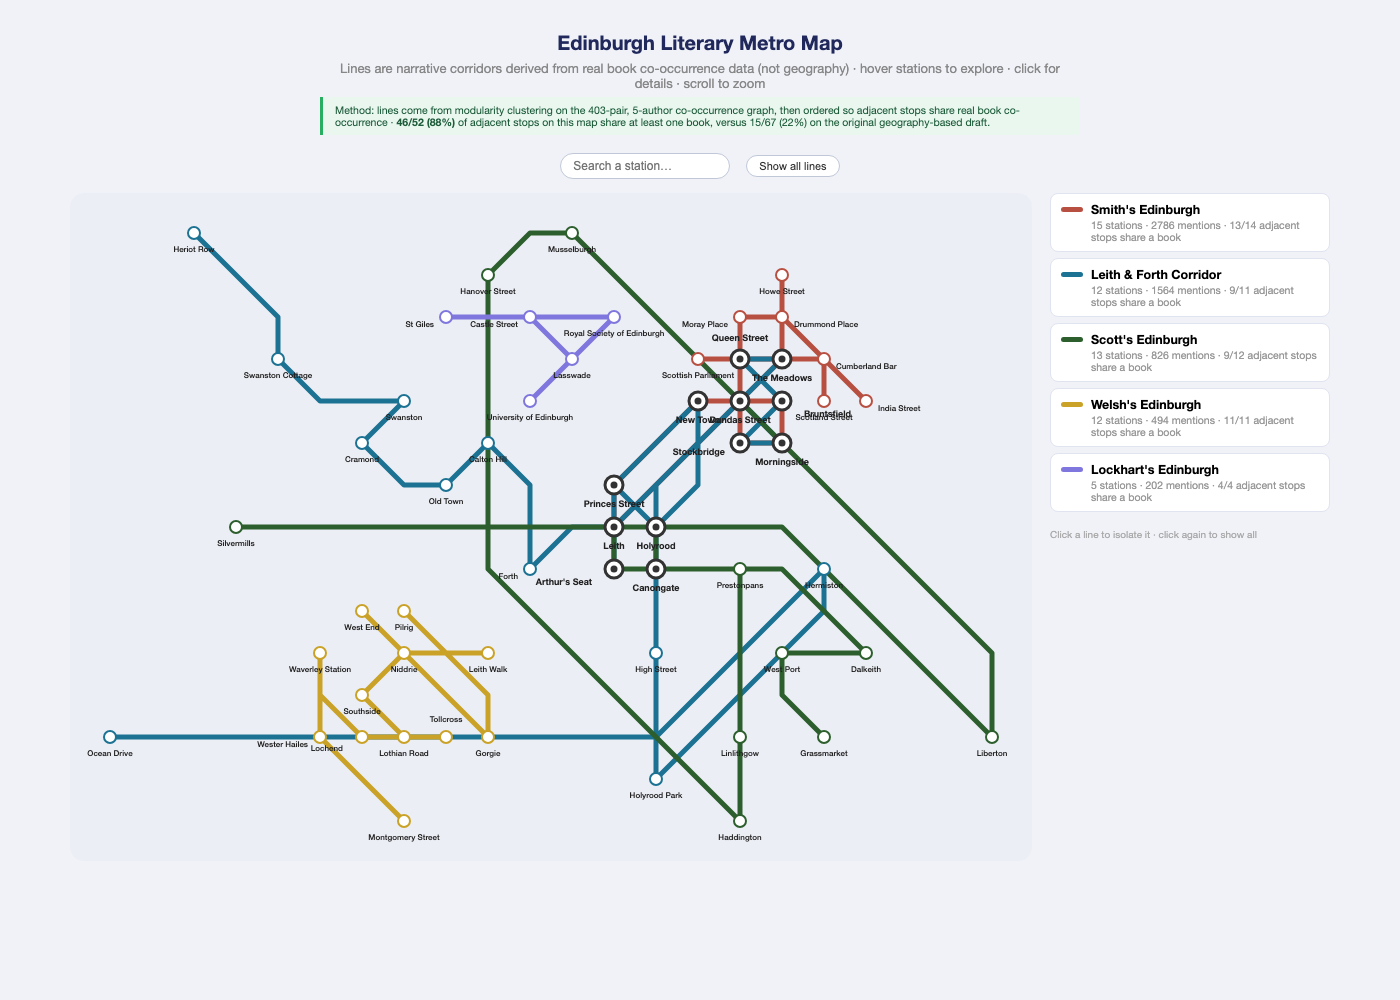
\includegraphics[width=0.55\textwidth]{figures/fig_metro.png}
\caption{The metro-style map after the redesign: five lines derived from modularity clustering on the co-occurrence graph and named after their dominant author, with 88\% of adjacent station pairs now backed by measured co-occurrence, against 22\% for the initial hand-drawn prototype (Figure~\ref{fig:metro-before}, Appendix~\ref{app:metro}).}
\label{fig:metro-after}
\end{figure}
 
\section{Design Summary}
 
Table~\ref{tab:design-summary} summarises the six visualisation designs and their key properties.
 
\begin{table}[h]
\centering
\caption{Summary of the six visualisation prototypes.}
\label{tab:design-summary}
\small
\begin{tabular}{llp{5cm}p{4cm}}
\toprule
Direction & Design & Primary encoding & Key interaction \\
\midrule
1 & Radar chart & Polygon shape across 14 sector axes & Click vertex for sector detail panel; example sentence on hover \\
1 & Bar-code & Bar height = mention share per place & Sector/frequency/alpha ordering; per-author Y-axis; search \\
1 & Small multiples & Bubble size on real map & Sync zoom; log/linear toggle; sector filter; 2-author compare mode \\
2 & Force-directed network & Node size = frequency; edge width = co-occurrence & Weight slider; drag nodes; click node for detail panel; absolute/percentage scale \\
2 & Linear connection & Arc height = node distance; arc width = weight & Weight slider; sort by frequency/sector/alphabet; click arc for book list; search \\
2 & Metro-style map & Line membership = community-detected narrative corridor & Click line to isolate; click station for detail panel; search \\
\bottomrule
\end{tabular}
\end{table}
 
 
% ============================================================
% CHAPTER 4: IMPLEMENTATION
% ============================================================
\chapter{Implementation}
\label{chap:impl}
 
\section{Data Pipeline}
 
\subsection*{Database setup}
 
PostgreSQL 16 was installed via Homebrew and a \texttt{litlong\_edinburgh} database created; the full LitLong dump (145\,MB, $\approx$2.3M lines) was imported directly via \texttt{psql}. This dump is more complete than the four CSV snapshots provided with the project brief (620 documents versus 548, 50,248 mention records versus 48,056, and 27 additional tables including \texttt{api\_sentence} and \texttt{api\_genre}). One table, \texttt{api\_location}, failed to import because its PostGIS geometry fields (\texttt{geom}, \texttt{poly}) require an extension that was not installed; it was instead imported from the CSV snapshot via Python/pandas, keeping only \texttt{id}, \texttt{text}, \texttt{lat}, \texttt{lon}, \texttt{gazref}, and \texttt{ptype}, since none of the visualisation directions need the geometry fields.

\subsection*{Narrative order extraction}

The \texttt{api\_locationmention} table's \texttt{start\_word} field encodes a global word index per mention, validated as strictly monotonically increasing within each document, so it can reconstruct reading order without parsing the source text. A custom table \texttt{mention\_order} was built with \texttt{word\_num} (extracted from \texttt{start\_word}), \texttt{mention\_order} (rank within document), and \texttt{position\_pct} (normalised position, $(\text{word\_num}-\min)/(\max-\min)$ per document), enabling Reader-plot style timeline visualisation as future work.

\subsection*{Sector classification}

The classification procedure is described in Section~\ref{sec:sectors}, implemented via the \texttt{shapely} library for point-in-polygon intersection against two GeoJSON boundary files from the City of Edinburgh Council's ArcGIS REST API (Neighbourhood Partnership Areas and Natural Neighbourhoods). Each place with a valid latitude/longitude was tested against the 14 sector polygons in order: an exact match if inside one, nearest-polygon assignment by Euclidean distance if within the bounding box but in an inter-polygon gap, and exclusion to a catch-all ``Outer Scotland'' category if outside the box entirely. Results were written to \texttt{location\_sectors} and exported as CSV.

\subsection*{Co-occurrence computation}

Document-level co-occurrence was computed in Python via \texttt{itertools.combinations}: for each document, every pair within its set of distinct places had its co-occurrence count incremented, filtered to weight $\geq 2$, yielding 403 pairs, exported as \texttt{network\_edges.csv} and \texttt{network\_nodes.csv}.

\subsection*{Sentence and book enrichment}

A second pass joins \texttt{api\_sentence} and \texttt{api\_document} to attach, for every place, a small sample of full source sentences (deduplicated, truncated to 220 characters, with book and author) and a ranked list of books that mention it; for Direction~2, the same join is computed per co-occurrence edge, so the places behind an arc or edge can be traced to the specific books where both appear. This is a separate lookup table keyed by place (and place pair), embedded alongside the existing data, and does not alter any previously computed percentage, count, or weight. Because sampling from \texttt{api\_sentence} surfaces source text verbatim, it can include informal register or strong language where the original does (e.g. Welsh's Scots-dialect prose) -- an authentic property of the corpus rather than a sampling artefact, but worth flagging before a live demonstration.

\section{Direction 1: Author Spatial Fingerprints --- Implementation}
 
\subsection*{Radar chart}

\begin{figure}[htbp]
\centering
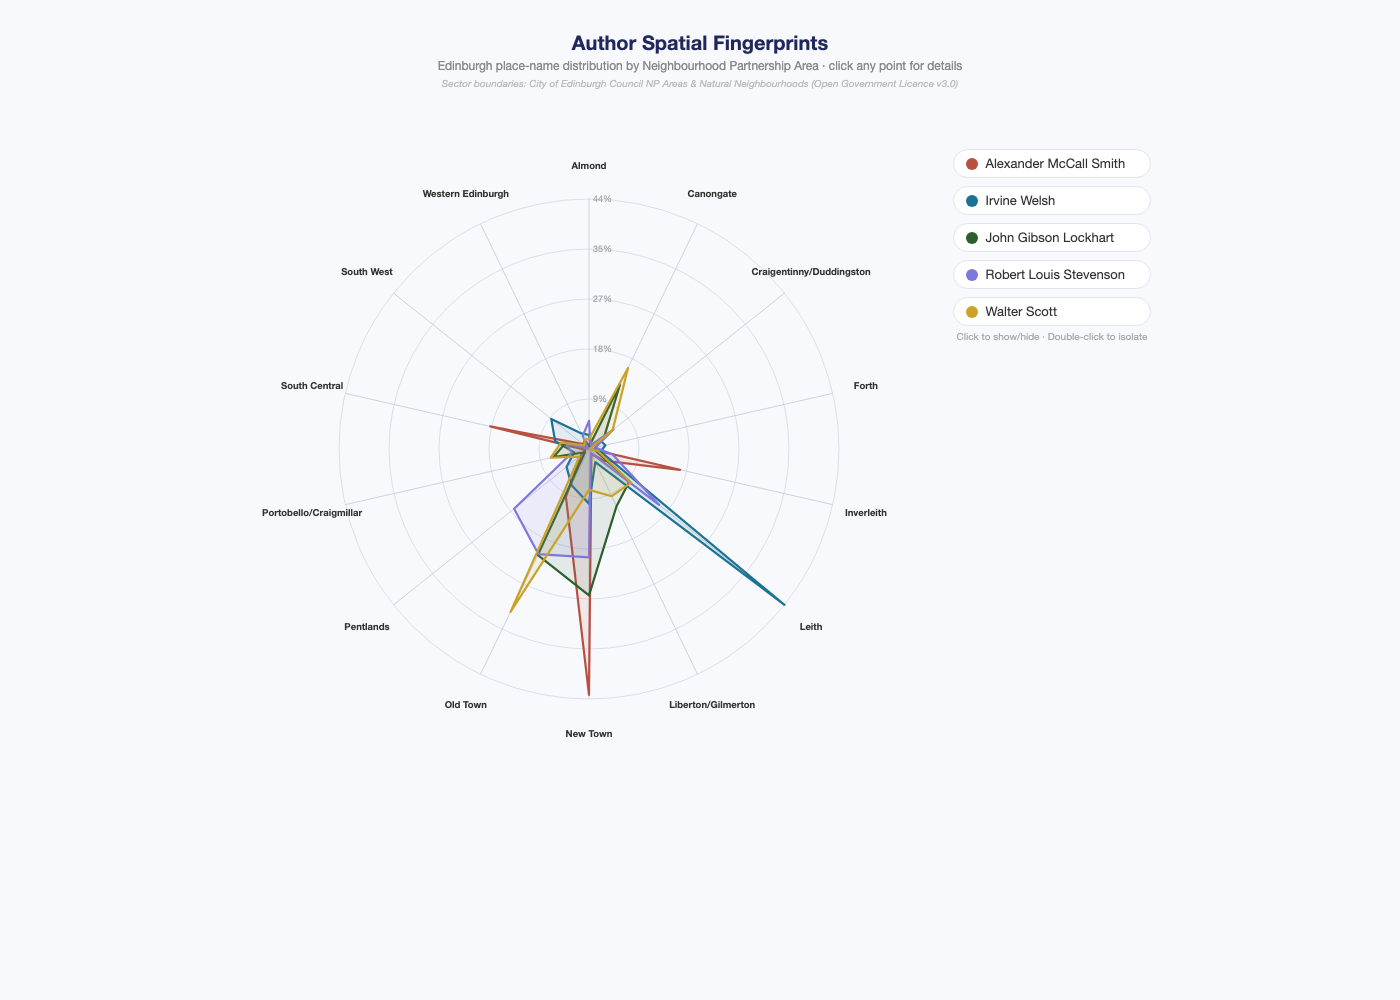
\includegraphics[width=0.55\textwidth]{figures/fig_radar.png}
\caption{The radar chart (primary Direction 1 design), showing all five test authors simultaneously. Each polygon is one author's distribution of place-name mentions across the 14 city sectors; the near-total lack of overlap between polygons is the visual evidence for the ``private imaginary geography'' finding reported in Section~\ref{chap:design}.}
\label{fig:radar}
\end{figure}

The radar chart is implemented using D3's \texttt{lineRadial} function with \texttt{curveLinearClosed}, which produces a closed polygon across the 14 angular positions. The angular spacing is $2\pi / 14$ radians per sector. The radial scale maps sector proportion to a radius between 0 and $R = 250$ pixels, where the scale maximum is set to the observed data maximum (0.436) rather than to 1.0.
 
Hover interaction uses invisible \texttt{circle} targets (radius 14px) centred on each vertex: a tooltip shows the sector name and percentage on hover, and a click opens a detail panel with the top eight places in that sector, ordered by mention count, plus a bar chart and the top five books. Data is embedded directly as JavaScript arrays in the HTML file, since browsers block \texttt{XMLHttpRequest} calls to local files under \texttt{file://} (a \texttt{d3.csv()} call would silently fail) -- the same approach used for all six visualisations.
 
\subsection*{Bar-code fingerprint}

\begin{figure}[htbp]
\centering
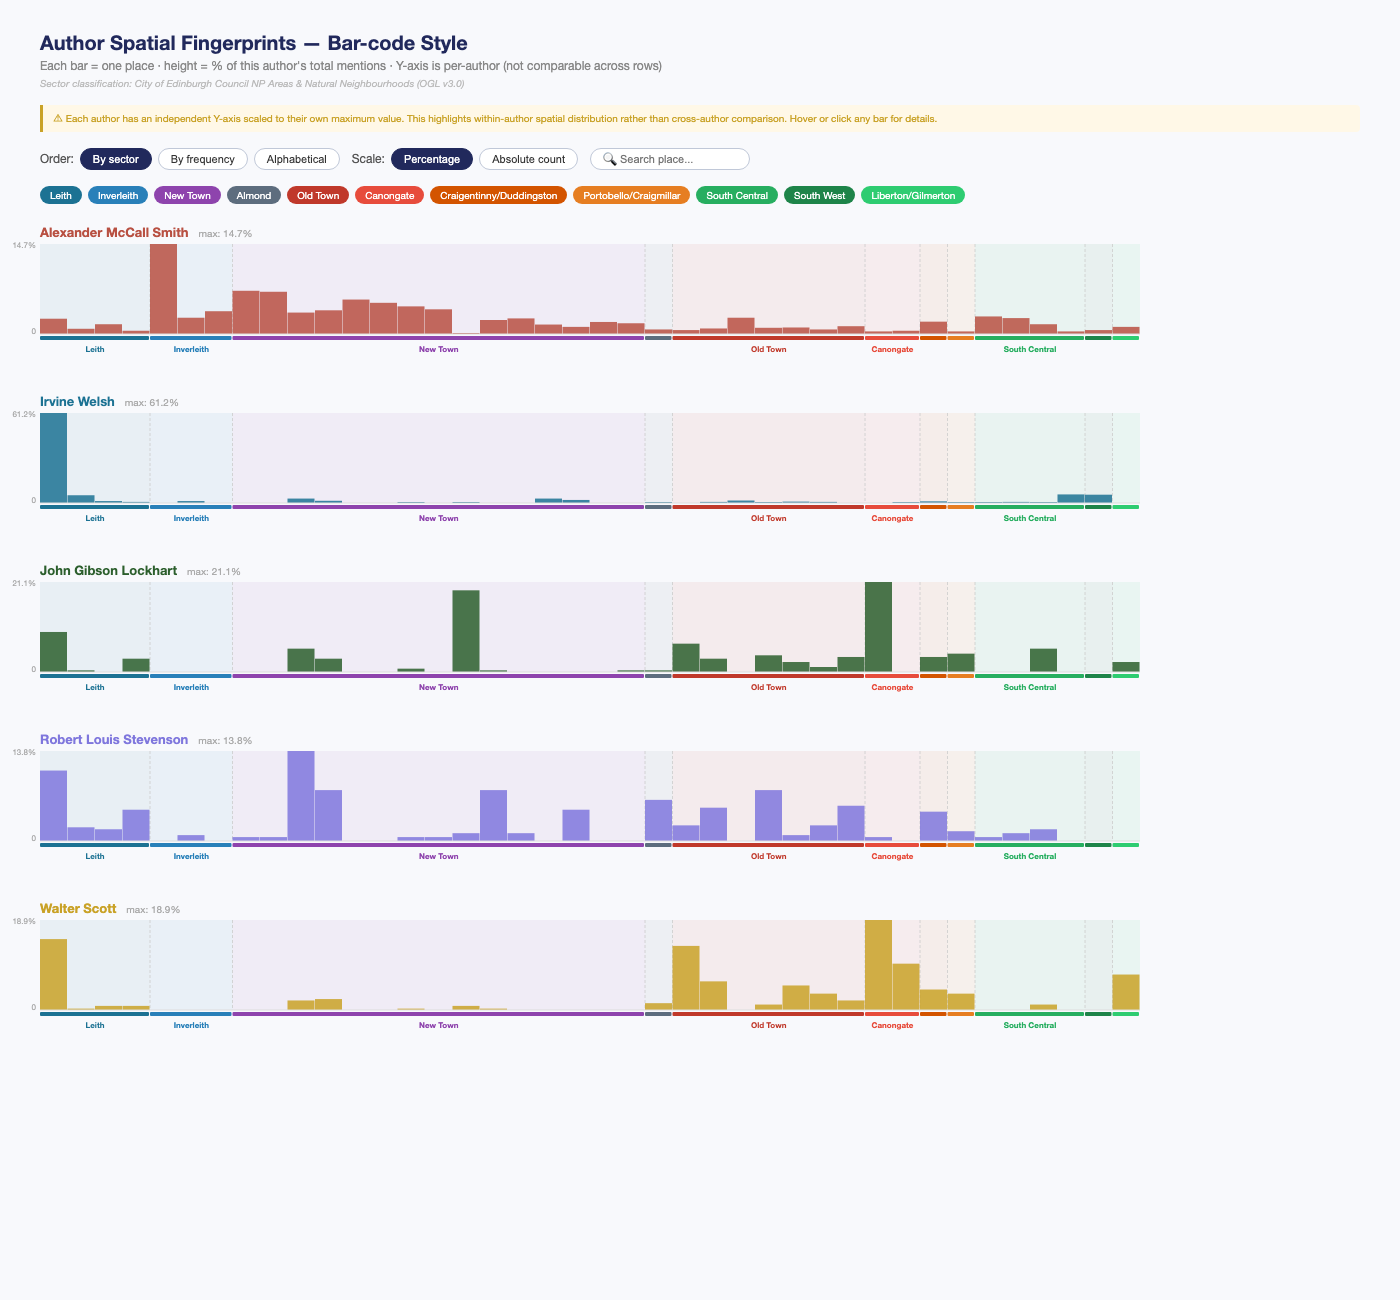
\includegraphics[width=0.55\textwidth]{figures/fig_barcode.png}
\caption{The bar-code fingerprint (secondary Direction 1 design). Each row is one author, each bar one place; bar height is normalised to that author's own maximum, so a short bar for a high-mention author is not visually confused with a tall bar for a low-mention author.}
\label{fig:barcode}
\end{figure}

Each author's row is an SVG element with Y-axis domain \texttt{[0, maxVal]}, where \texttt{maxVal} is that author's own maximum proportion rather than the global maximum -- the deliberate per-author scaling justified in Section~\ref{chap:design}.
 
Sector boundaries use two complementary encodings: a low-opacity background rectangle spans the bars in each sector, and a narrow colour strip below the bar area identifies it, with text labels shown only where a sector is wide enough to hold them (threshold 40px) to avoid label stacking. Switching between ordering modes (sector, frequency, alphabetical) and scale modes (percentage, absolute) re-renders the SVG elements with the new ordering applied, rather than animating existing elements, which avoids the complexity of D3 transition management across multiple SVG groups.
 
\subsection*{Small multiples}

\begin{figure}[htbp]
\centering
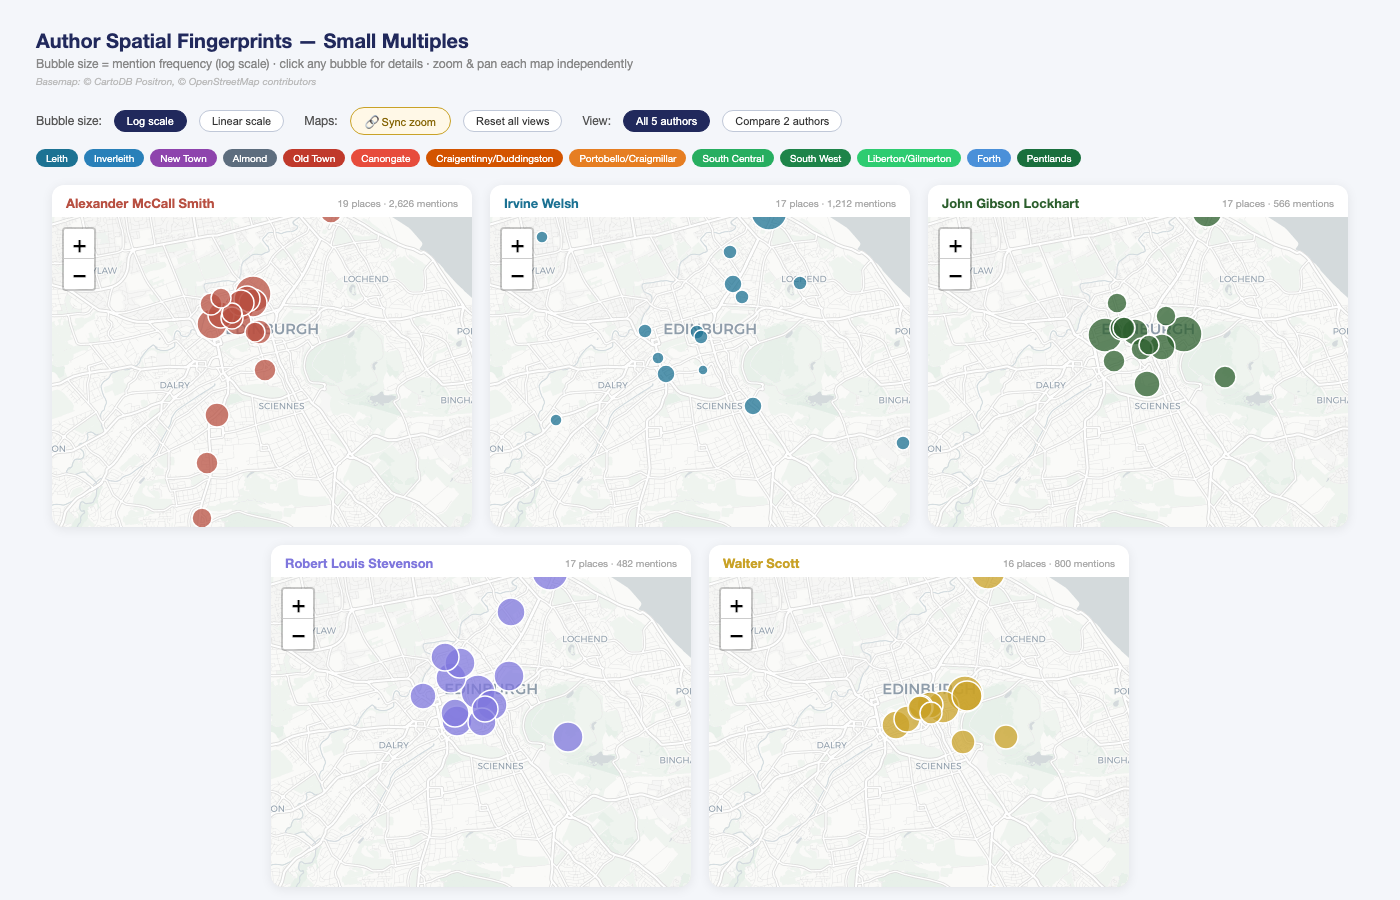
\includegraphics[width=0.55\textwidth]{figures/fig_small_multiples.png}
\caption{The small multiples design (tertiary Direction 1 design), five independent Leaflet maps side by side. Unlike the other two Direction 1 designs, this one retains real geographic coordinates as a spatial anchor, at the cost of the visual comparison being harder to make at a glance across panels.}
\label{fig:small-multiples}
\end{figure}

Each of the five panels is an independent Leaflet.js map instance (CartoDB Positron tiles), with place-name bubbles as Leaflet \texttt{CircleMarker} objects whose radius recomputes on scale-mode change; this replaced an earlier two-stage Leaflet/D3 overlay that required manual screen-coordinate projection and did not handle pan/zoom correctly. Synchronised zoom attaches a \texttt{moveend} listener to each map that calls \texttt{setView} on the others when the sync toggle is enabled, guarded by an \texttt{isSyncing} flag against cascading updates.
 
\section{Direction 2: Narrative Topology --- Implementation}
 
\subsection*{Force-directed network}

\begin{figure}[htbp]
\centering
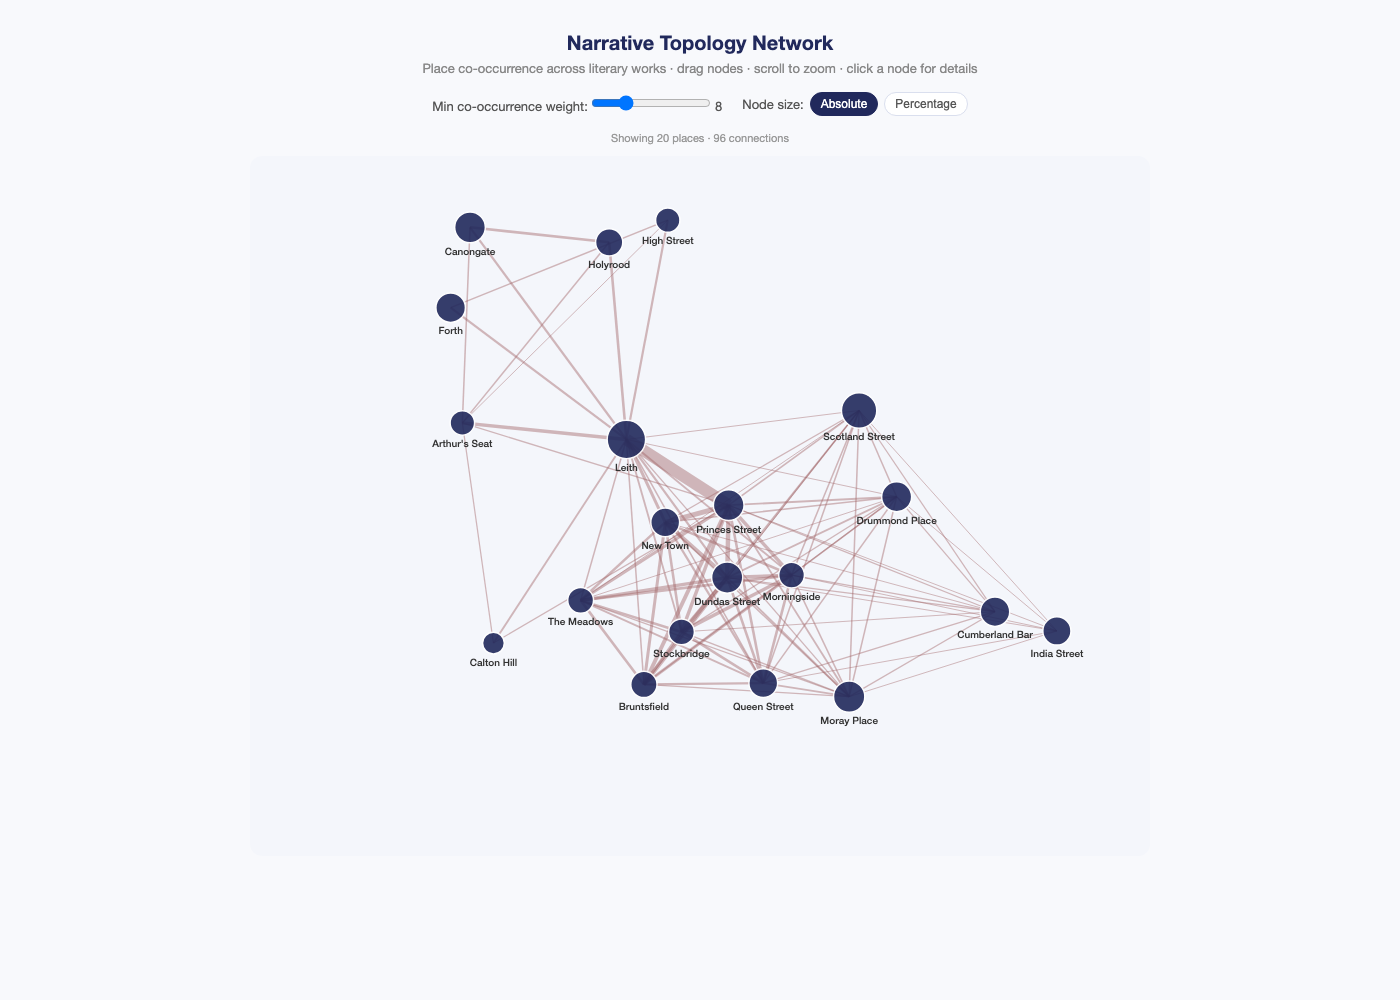
\includegraphics[width=0.55\textwidth]{figures/fig_network.png}
\caption{The force-directed network (primary Direction 2 design). Nodes are places, edges are document-level co-occurrence; node size reflects mention count. Leith and Princes Street, the strongest co-occurring pair in the corpus, are visibly pulled together despite the roughly 2.5km geographic distance between them.}
\label{fig:network}
\end{figure}

The simulation uses four forces: \texttt{forceLink} (spring attraction, distance inversely proportional to weight), \texttt{forceManyBody} (uniform repulsion, strength $-400$), \texttt{forceCollide} (collision avoidance, node radius + 18px), and \texttt{forceCenter} (gentle centring). It re-runs from scratch on each weight-threshold change, since the active node/edge set changes and a smooth topology transition is not meaningful. Node labels sit at $y = \text{node.y} + r + 12$px, below each node; an earlier centroid placement with white fill was invisible against the equally dark node background.
 
\subsection*{Linear connection diagram}

\begin{figure}[htbp]
\centering
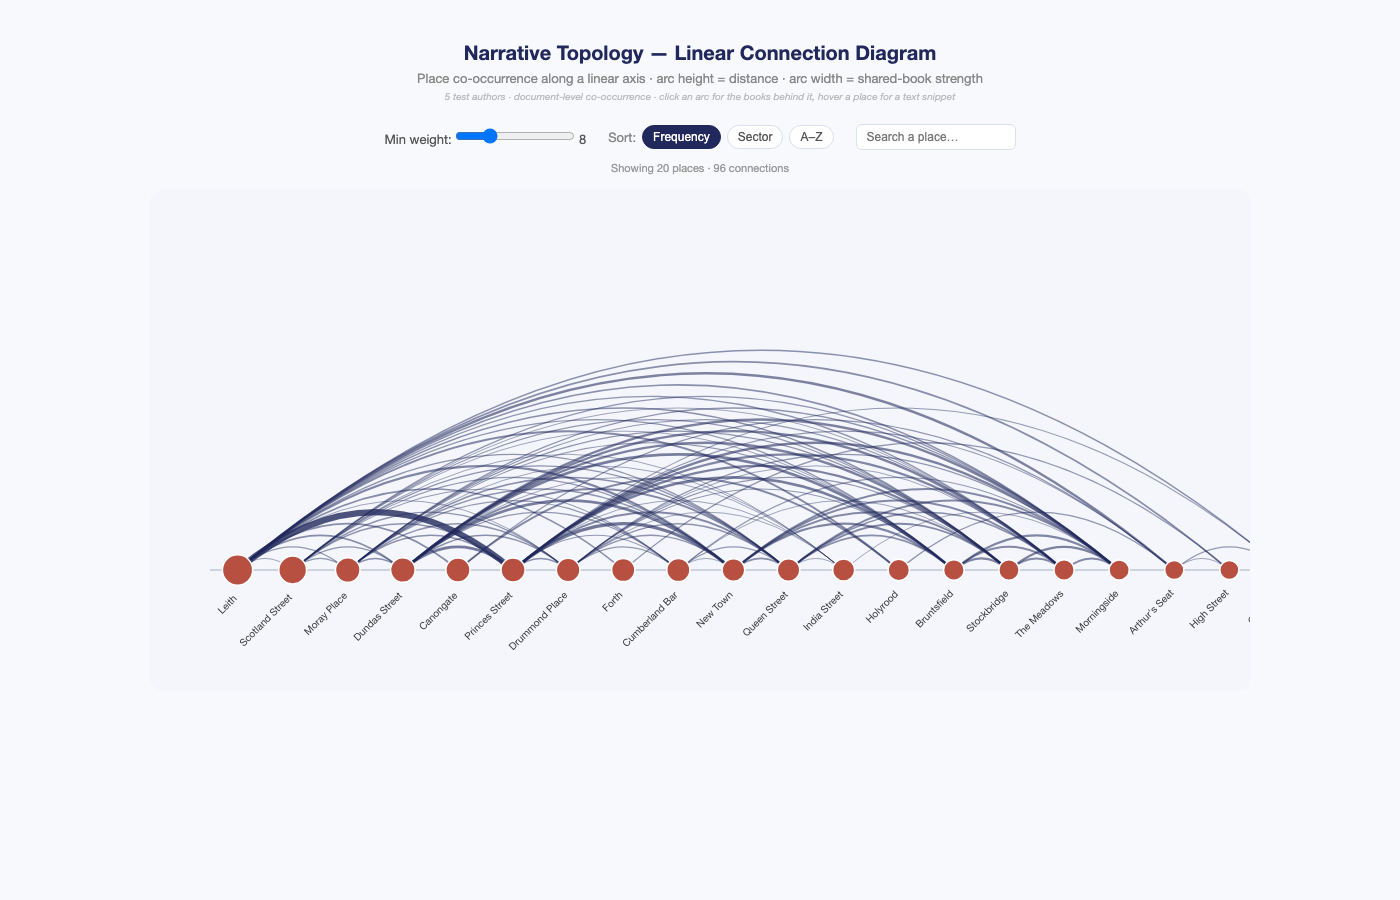
\includegraphics[width=0.55\textwidth]{figures/fig_linear.png}
\caption{The linear connection diagram (secondary Direction 2 design). Places sit on a single horizontal axis; arc height and thickness both encode co-occurrence weight, so the strongest connections are immediately visible as the tallest arcs regardless of how far apart their endpoints are on the axis.}
\label{fig:linear}
\end{figure}

Each arc is drawn as a quadratic Bézier path: \texttt{M x1 y0 Q midX (y0 - h) x2 y0}, where \texttt{midX} $= (x1 + x2) / 2$ and \texttt{h} $= |x2 - x1| \times 0.42$. The coefficient 0.42 was chosen to produce arcs that are visually distinct without extending beyond the SVG canvas for the longest connections. Stroke width is computed as $(w / w_{\max})^{1.5} \times 6$.
 
\subsection*{Metro-style map}

\begin{figure}[htbp]
\centering
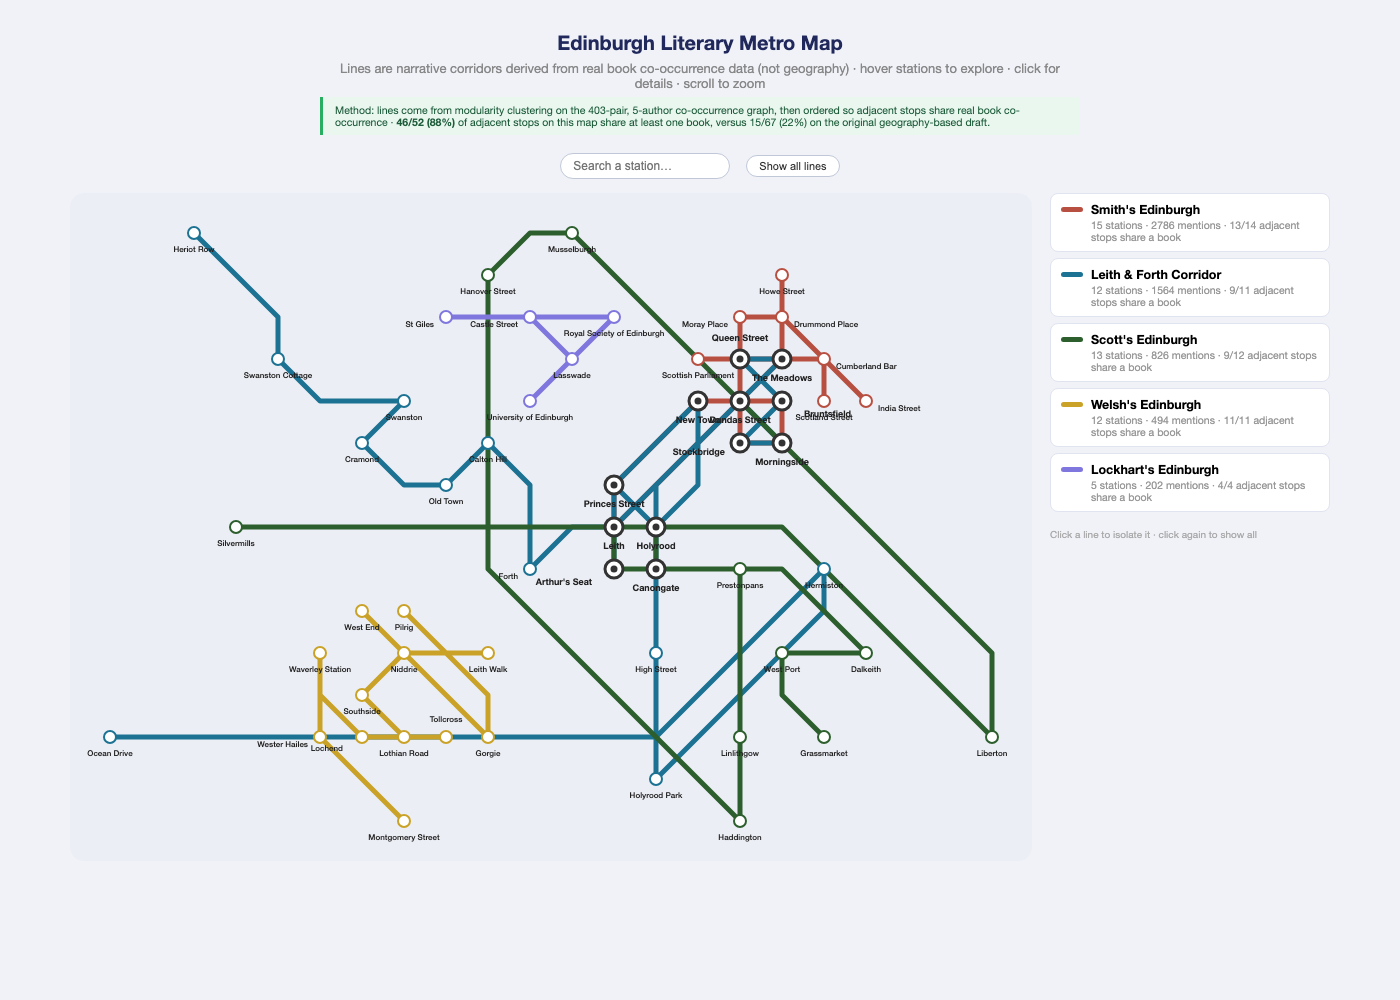
\includegraphics[width=0.55\textwidth]{figures/fig_metro.png}
\caption{The metro-style map (illustrative Direction 2 design) after the data-driven redesign described in Section~\ref{sec:metro-redesign}. Lines are named after their dominant author and derived from modularity clustering on the co-occurrence graph, not drawn by hand; interchange stations (double-ringed) mark places that multiple authors' narrative corridors both pass through.}
\label{fig:metro}
\end{figure}

The redesigned pipeline (Section~\ref{sec:metro-redesign}) is implemented as two Python scripts: \texttt{build\_metro\_lines.py} performs the community detection, station sequencing, interchange detection, and layout, writing a JSON file with each line's name, colour, member stations, shared grid coordinates, and adjacency-backed diagnostic count; \texttt{build\_metro\_html.py} consumes this JSON and renders the HTML file. Separating derivation from rendering means the clustering parameters can be adjusted and the map regenerated without touching the rendering code.

Python's hash-randomised set/dictionary iteration means \texttt{greedy\_modularity\_communities} can break ties differently between runs, changing station sequencing along a line (though not line assignment); running with \texttt{PYTHONHASHSEED=0} fixes this and was adopted as standard practice.

At render time, each line is drawn as an SVG path through its stations' shared grid coordinates, pixel-converted and octilinearity-corrected as described in Section~\ref{sec:metro-redesign}. Because coordinates are shared across lines, two lines meeting at the same interchange are drawn through the same physical point, producing genuine crossings rather than the separate parallel lanes of the initial prototype. Interchange stations follow the London Underground convention (outer white ring, inner dark circle); the greedy label-placement search reduced overlapping label pairs among the 57 stations from ten to two. D3 zoom supports scroll-to-zoom and drag-to-pan; clicking a line or legend entry isolates it, and a text field highlights matching stations.
 
\section{Technical Decisions and Constraints}
\label{sec:technical-decisions}

\textbf{Data embedding.} All six D3 HTML files embed their data as JavaScript object literals -- larger file sizes and a regeneration step on data change, an acceptable constraint for a research prototype evaluated on a fixed dataset.
 
\textbf{Versioning and compatibility.} Each HTML file is versioned under filenames such as \texttt{radar\_v1.html}, a record of the design evolution. All files were tested in Safari and Chrome on macOS; D3.js v7 and Leaflet.js 1.9.4 load from CDN at runtime, requiring an internet connection.

\textbf{Colour accessibility.} The five fixed per-author colours were checked against simulated protanopia, deuteranopia, and tritanopia (the Brettel/Vi{\'e}not transform) rather than assumed distinguishable. All ten pairs remain separable under all three; the closest, McCall Smith and Scott, is still above the confusion-risk threshold used here. The palette is reasonable but not maximally optimised, since colours were originally chosen for interface contrast rather than colour-vision-deficient legibility specifically.
 
\section{Combined Interface}
\label{sec:combined-interface}

The combined interface (\texttt{data/processed/combined/d3/combined\_interface.html}) is a supplementary exploration tool, not part of the formal user study reported in Chapters~\ref{chap:eval}--\ref{chap:discussion}: it puts all six designs behind one shared author selector (presets for 2/5/20/50/408 authors, free-text search, or a full custom checklist), reusing the client-side computation already built for the scale exploration (Appendix~\ref{app:scale}). Five views (radar, bar-code, small multiples, network, linear) re-render live from the current selection; clicking an author in a fingerprint view highlights their places in a topology view via a shared \texttt{focusedAuthor} value, and a unified detail panel shows an example sentence and book list for whatever is hovered. The metro map is the one exception, since its lines depend on offline community detection (Section~\ref{sec:metro-redesign}) rather than a per-keystroke computation, so it switches between five precomputed snapshots (2/5/20/50/408 authors) instead of recomputing live.

Building this tool surfaced one finding that carries beyond the interface itself: at the 50-author preset, the live co-occurrence graph reaches 12,833 edges, enough that D3's force simulation failed to settle and the interface became visibly unresponsive until rendering was capped to the 1,500 strongest-weighted edges. This is the same density-versus-scale trade-off already reported for the standalone scale-exploration tool (Section~\ref{sec:limitations}), now confirmed as a real interactivity constraint rather than only a static-rendering one.
 
% ============================================================
% CHAPTER 5: EVALUATION
% ============================================================
\chapter{Evaluation}
\label{chap:eval}
 
\section{Study Design}
\label{sec:study-design}

The user study is designed to evaluate whether the six visualisation prototypes support the tasks implied by the two research questions: author identification (RQ1) and narrative-relationship identification (RQ2).
 
\textbf{Participant groups.} Two groups were recruited: domain experts (literary scholars, digital humanists, and researchers familiar with Edinburgh's literary geography) and general public, to test whether expert and non-expert users differ in which design they find most legible and in whether they spontaneously perceive the narrative/geographic divergence.

\textbf{Format.} The study was conducted online, unmoderated and self-paced, to maximise recruitment reach and to have participants interact with the visualisations in a real-world browser environment.

\textbf{Introduction protocol.} Participants saw each visualisation with only a brief description of the project's purpose, no explanation of the encoding or how to read it. This ``cold'' presentation tests whether the designs are self-explanatory, rather than participants' ability to apply an explanation they were given -- a participant who needs the design explained is, in effect, reporting a usability problem. This differs from the labelled reference view in Task~1 below, which gives participants something to look at before being tested, without telling them what to look for.
 
\textbf{Tasks.} Two task types are used. Task~1 (fingerprint direction) tests the RQ1 success criterion from Chapter~\ref{chap:intro} -- whether the fingerprint shapes are distinct enough to be learned and recognised, not whether a participant can name an author from memory of their books -- via a study-then-identify structure. Participants first see a labelled reference view (all five authors' fingerprints together, the canonical prototype from Chapter~\ref{chap:design}) and spend a few minutes noticing how the shapes differ, unprompted. They then see a single-author blind variant with the legend and detail panel removed (which would otherwise expose book titles) and rendered in a neutral colour rather than the author's own, guarding against answering from a remembered colour swatch rather than the shape itself, and are asked which author it represents. To guard against a participant matching the outline from memory without engaging with what it communicates, the task opens with an objective, answer-keyed question -- which sector or place the shape indicates the author writes about most -- answerable only from the blind stimulus itself; the accompanying open-text question on what feature led to that answer is treated as equally important, since it captures reasoning even when the forced-choice answer is wrong. A different author is used per design to avoid anchoring across the three fingerprint tasks. Because a single blind identification only yields a one-in-five correct/incorrect judgement, Task~1 adds a third step: matching all five unlabelled, shuffled shapes to authors, producing a full $5\times5$ confusion matrix per design plus a self-rated confusability judgement. Both task directions also guard against ceiling/floor effects on their primary measures: Task~1 adds a runner-up guess and a forced choice between the single most confusable author pair per design (identified in advance by cosine similarity on the data); Task~2 adds ratings of three place pairs of known strong/medium/weak co-occurrence weight and a forced choice between a real data-derived cluster and two constructed distractors (full wording in Appendix~\ref{app:questionnaire}). Task~2 (topology direction) shows a topology visualisation and asks participants to identify the two most strongly connected places and judge whether they are geographically close or far; since all three topology designs already show every place labelled in one aggregated structure, no reference-then-blind structure is needed, and the secondary question tests whether the design spontaneously communicates the narrative/geographic divergence finding. After completing all tasks, participants vote for the most intuitive design in each direction.
 
\textbf{Ethics.} The study has received ethics approval from the Informatics Research Ethics Committee (application number 446635). Participants complete an online consent form before beginning the study. The participant information sheet and consent form are included in Appendix~A.
 
\section{Participants}

Sixteen responses were collected; three were excluded on data-quality grounds (Section~\ref{sec:study-procedure}), leaving $n=13$. Participants were recruited through the researcher's personal and academic network within the UK, per the eligibility criteria in the approved ethics application, not restricted to the University of Edinburgh.

Grouping into ``domain expert'' and ``general public'' was based on self-described background (Q-B3) rather than assigned at recruitment (Section~\ref{sec:study-design}): four participants reporting a background in literary studies, digital humanities, or visualisation/HCI/computer science formed the expert group, the remaining nine the general-public group -- thinner on the expert side than the five-to-eight target, so treated throughout as exploratory rather than statistically powered.

A striking feature of the sample, expert group included, is near-uniform unfamiliarity with the five specific authors: nine of thirteen had read none of them, and eight rated themselves ``not at all familiar'' with Edinburgh's literary history, including the one literary-studies participant. This is not a recruitment weakness but a confirmation that the identification tasks (Section~\ref{sec:fp-results}) test whether the encoding itself is learnable, not prior author knowledge. General visualisation-reading familiarity was more evenly spread (``moderately familiar'' most common); four participants had lived in Edinburgh, one had visited, eight never had.

\section{Study Procedure}
\label{sec:study-procedure}

The study was distributed as an anonymous Qualtrics link, completed online, unmoderated, and self-paced. Median completion time among the retained responses was 46 minutes, in line with the estimated 50--65; the wider recorded range reflects Qualtrics' ``finish later'' option letting some participants leave the survey open across more than one sitting, inflating elapsed but not active time.

Three of sixteen raw responses were excluded: one completed in under ten minutes with near-empty free text (a single full stop in place of an explanation); one gave single-letter, non-committal answers (``a'', ``b'', ``no'') on every free-text field, including the anti-memorisation questions (F0, T1b) that specifically ask for justification; one completed in six minutes with free text unrelated to the questions asked. All three were judged not to reflect genuine engagement and excluded before analysis. A small number of retained free-text answers, originally given in Chinese by UK-resident participants, are translated by the researcher and reproduced alongside the original wording rather than replacing it.

\section{Results}
\label{sec:fp-results}

\textbf{Fingerprint identification and matching (RQ1).} Results below are reported per design, out of $n=13$, with the single-author identity used for the blind stimulus given in parentheses.

\emph{Radar chart (Walter Scott).} The encoding-legibility check (F0) was answered correctly by 10/13 participants (77\%), the highest of the three designs. Single-shape identification (F1) was correct for 6/13 (46\%), rising to 8/13 (62\%) once a correct second guess (F1b) is credited. On the five-way matching task (M1), 45 of 65 shape-to-author assignments were correct (69\%, against a 20\% chance baseline), the highest matching accuracy of the three designs; the most common confusions were between Robert Louis Stevenson and Irvine Welsh, and between John Gibson Lockhart and Robert Louis Stevenson. On the targeted hardest-pair check (P1, Lockhart vs Scott), 11/13 (85\%) correctly distinguished the two.

\emph{Bar-code (John Gibson Lockhart).} F0 was correct for 6/13 (46\%). F1 was correct for 6/13 (46\%), rising to 10/13 (77\%) on the Top-2 measure, the largest Top-1-to-Top-2 gain of the three designs, consistent with participants narrowing the shape to a plausible pair without landing on the exact author. M1 matching accuracy was 31/65 (48\%); the most frequent confusions were between Robert Louis Stevenson and John Gibson Lockhart, and between Irvine Welsh and Walter Scott. P1 (Scott vs Welsh) was correct for 10/13 (77\%).

\emph{Small multiples (Robert Louis Stevenson).} This design produced the weakest results on every fingerprint measure: F0 correct for 5/13 (38\%), F1 for 3/13 (23\%), Top-2 for 5/13 (38\%), and M1 matching accuracy 32/65 (49\%), with Walter Scott the author most often confused for others. P1 (Lockhart vs Stevenson) was nonetheless correct for 10/13 (77\%), comparable to the other two designs, suggesting that even where overall identification is weak, the single most-confusable pair is not disproportionately harder here than for the stronger designs.

Self-explanatoriness (F4, ``would you have understood this without explanation'') was mixed for all three designs, with no design rated ``yes, easily'' by more than a third of participants. In the post-task ranking, the three fingerprint designs were close to an even three-way split (small multiples 5 votes, radar chart 4, bar-code 4).

\textbf{Narrative topology (RQ2).} All three topology designs share the same underlying co-occurrence data, so the same ground-truth pair (Leith and Princes Street) and design-specific place pairs/clusters documented in Appendix~A apply throughout.

\emph{Force-directed network.} T1 (identify the strongest pair) was correct for 9/13 (69\%). Ratings on the three fixed strength-check pairs (T-Strength) correlated strongly with the pairs' real co-occurrence weights ($r=0.64$, $p<0.001$, $n=39$ ratings), the strongest correlation of the three designs. T-ClusterVerify was correct for 9/13 (69\%), matching T1's accuracy.

\emph{Linear connection diagram.} T1 was also correct for 9/13 (69\%), identical to the network. The strength-rating correlation was weaker and not conventionally significant ($r=0.30$, $p=0.067$, $n=39$). T-ClusterVerify accuracy was markedly lower than the other two designs at 3/13 (23\%); the large majority (8/13) instead selected a distractor grouping (New Town, Leith Walk, Holyrood, Waverley Station) built by deliberately mixing places from different real communities, suggesting the linear diagram's arc-based encoding does not communicate cluster membership as clearly as the other two designs, despite matching them on the single strongest-pair task.

\emph{Metro-style map.} T1 accuracy was substantially lower than the other two designs at 2/13 (15\%), even though the same underlying pair is, by construction, the single strongest edge in every design. The strength-rating correlation was weak but statistically significant ($r=0.34$, $p=0.035$, $n=39$). T-ClusterVerify accuracy was 7/13 (54\%), between the other two designs. Despite this being the weakest design on two of the three objective measures, it was the clear winner of the post-task ranking (7/13 votes, against 5 for the network and 1 for the linear diagram), and of the final ``most memorable visualisation'' question (Q-R5) among those who named a specific design.

\section{Discussion of Results}

The clearest single result is that the radar chart outperforms the other two fingerprint designs on every measure: F0 comprehension, single-identification and Top-2 accuracy, five-way matching, and hardest-pair discrimination. This matches the qualitative pattern in F3 answers, where radar-chart responses often named a specific sector (``a very large spike in Leith area'', ``the maximum is old town''), while bar-code and small-multiples answers more often described a feature without naming it (``peak value''). The polygon's asymmetry appears to give participants a concrete verbal handle the other two encodings did not as reliably provide; since F0 accuracy tracks F1 accuracy design-for-design, this supports F0 as a genuine engagement check rather than a proxy for shape memorability alone.

Small multiples' weak performance across F0, F1, and M1 is notable given it is the most visually distinctive design at the reference-viewing stage (five separate maps): that distinctiveness evidently did not transfer to the blind, isolated shape. All three designs nonetheless cleared the P1 hardest-pair check well above chance (77--85\%), and the gap between M1 and P1 for small multiples specifically (49\% vs 77\%) indicates its difficulty lies more in distinguishing all five patterns at once than in any single pairwise comparison.

For topology, the network and linear diagram matched on the single strongest-pair task (69\% each) but diverged sharply on cluster recognition (network 69\%, linear 23\%, barely above the 33\% random baseline). Read with the network's stronger strength-rating correlation ($r=0.64$ against $r=0.30$), this points to one difference: encoding strength as edge thickness and spatial proximity communicates both a strongest pair and a broader cluster more reliably than arc height along a single axis, even though the two are statistically indistinguishable on the narrower single-pair task.

The metro map is the most interesting tension in the results: worst of the three on the strongest-pair task (15\%, against 69\% for the others) despite encoding the same weight in its line structure, yet decisively the most popular in the post-task ranking and most-named ``most memorable'' design. Participants' own explanations (``similar to real transit maps I am familiar with'', ``its like a map that we see everyday'') suggest its borrowed visual language reads fluently as a familiar transit map rather than as an instrument for locating one specific edge -- confident navigation, not task accuracy. This is an unintended illustration of the same trade-off Beck's Underground map itself makes (Section~\ref{sec:direction2}): a comfortable, generalisable mental model of the whole network over precise retrieval of any single edge weight.

Cross-tabulating by expert/general-public group carries the caveat, restated because it matters, that four experts is too small a group for a robust comparison (a single answer shifts the expert percentage by 25 points). Descriptively, expert free-text answers were not obviously more accurate, but more often referenced the underlying literary-geographic content directly: one expert's synthesis answer, ``I was surprised that some places that are geographically quite separate still seem closely connected in the authors' writing. It made me realise that literary connections between places do not necessarily follow their physical locations,'' restates the dissertation's own RQ2 argument unprompted, and another's, ``Yes, Walter Scott in Leith I did not realise this is where his work was set,'' is a direct instance of the visualisation surfacing an unknown literary fact. Both are treated as indicative rather than representative given the sample size, but are the kind of qualitative evidence the deep-insight questions (T3, T4, Cross-design synthesis) were designed to surface.
 
 
% ============================================================
% CHAPTER 6: DISCUSSION
% ============================================================
\chapter{Discussion}
\label{chap:discussion}
 
\section{Design Improvements after User Study}

The results in Section~\ref{sec:fp-results} point to concrete, design-specific changes rather than one across-the-board fix, since each design failed, where it failed, differently.

For small multiples, the weakest performer on every objective measure, the gap between strong reference-view distinctiveness and weak blind-identification accuracy suggests the problem is the loss of side-by-side comparison rather than legibility in the abstract: a faint, unlabelled silhouette of the other four authors' spatial envelopes in the blind view is worth testing, preserving comparison without reintroducing identity. For bar-code, the large Top-1-to-Top-2 gain (46\% to 77\%) suggests participants extract real signal without a reliable way to commit to one answer; defaulting to frequency rather than sector ordering, already several participants' stated F3 strategy, may make the largest bar easier to commit to.

For topology, the metro map's weak strongest-pair accuracy despite strong subjective preference is the clearest case for a targeted change: since its transit-map familiarity is a genuine strength worth keeping, a lightweight strength cue within that visual language (line thickness, or station size proportional to interchange weight) is more promising than abandoning the metaphor. The linear diagram's poor cluster recognition (23\%, barely above the 33\% chance baseline) despite matching single-pair accuracy suggests its single-axis layout communicates one connection well but not multi-place groupings; arc-bundling or community-membership colour-coding would give it an explicit cluster cue it currently lacks.

More generally, F0's correlation with F1 accuracy across all three fingerprint designs suggests future iterations could use F0-style objective legibility checks earlier in the design process, catching a distinctive-looking but non-communicative design before a full user study is built around it.
 
\section{Narrative Topology vs Geographic Topology}
 
The most striking finding from the data analysis is the co-occurrence of Leith and Princes Street across 28 distinct literary works, the strongest pair in the entire corpus, despite sitting roughly 2.5 kilometres apart: Leith a port district historically tied to trade and working-class life, Princes Street the commercial artery of the bourgeois Georgian New Town. On a geographic map they are simply two points in the same city; in the narrative topology visualisation they are the closest pair in the network. One plausible reading is that the journey between them recurs as a structuring device in Edinburgh fiction because it crosses a social as well as a spatial boundary, a pattern consistent with Irvine Welsh's \textit{Trainspotting} (Leith and the city centre as a crossing between social worlds) and Scott's historical novels (the Old Town closes and the wider city as a crossing between historical strata) -- though this dissertation's corpus analysis measures co-occurrence rather than the social or narrative content of that journey, so the interpretation is offered as a literary reading of the pattern, not a claim tested directly by the data. A geographic map cannot show this; the narrative topology visualisation shows these two places as \emph{narratively adjacent} regardless of spatial distance. The finding speaks directly to Westphal's geocriticism, which argues literary space is relational and constructed rather than a reflection of physical geography \cite{westphal2011}: the places most strongly connected in Edinburgh's literary imagination are not the places nearest each other on a map.

The metro-map redesign (Section~\ref{sec:metro-redesign}) offers a related but methodologically distinct observation: an internal-consistency check rather than an independent test of the claim above, since the redesigned lines are themselves derived from the co-occurrence graph and are then checked against that same graph. Read this way, the result is still informative -- only 22\% of the hand-drawn map's same-line adjacencies were backed by real co-occurrence, against 88\% once lines were derived from the graph itself -- but as evidence that a co-occurrence-optimised grouping is more internally consistent with the underlying data than a geography-optimised one, consistent with Finding~4, rather than as a second independent demonstration that narrative topology diverges from geography (the Leith/Princes Street finding above, which compares co-occurrence against an unrelated measure, geographic distance, is the independent evidence for that claim). The redesign also surfaced two findings the geographic version could never have produced. Leith, as a place name across all five authors combined, groups with the historical Old Town corridor of Scott and Lockhart rather than with the contemporary, working-class Leith of Welsh's novels -- a finding about how the name functions across a corpus rather than about any one author's usage, visible only once co-occurrence rather than individual usage is what groups places. Separately, a five-station corridor (Castle Street, Lasswade, the University of Edinburgh, the Royal Society of Edinburgh, and St Giles) emerged as a coherent cluster corresponding to Lockhart's biographical rather than fictional geography of Scott -- places he lived and worked, per \textit{Life of Walter Scott}, not places his novels are set -- distinguishing this biographical register from the historical-fiction register of the neighbouring Old Town corridor without being told to.

\section{Author Spatial Languages}
 
The near-total absence of shared place names across the five test authors (zero shared by three or more, only 18 by any two) can be stated as a simple number but deserves interpretation: each author has constructed an Edinburgh that is almost entirely their own -- McCall Smith's bounded by the Scotland Street/Dundas Street/Drummond Place triangle in the New Town, Welsh's by Leith, Scott's by the Canongate and Old Town closes, Stevenson's extending to the Pentlands (his childhood at Swanston Cottage) and the Firth of Forth (his father's lighthouse engineering). The radar chart and bar-code fingerprint make these private geographies comparable at a glance -- a user who knows nothing of these authors' biographies can see, from polygon shape alone, that McCall Smith and Welsh occupy different spatial territories within the same city, encoding in geometry an argument that would otherwise require paragraphs of prose.

This vocabulary separation also explains a non-obvious pattern from scale-testing the network graph against the full corpus (\texttt{network\_scale\_explore.html}): co-occurrence density does not fall smoothly as author count grows, but is high at both the very small end (two authors, or two-to-three books) and low at the very large end (408 authors), for two related reasons. At the small end, document-level co-occurrence approaches its degenerate case, since almost any two places in a handful of books will co-occur at least once; three books (two by McCall Smith, one by Welsh) produced 152 places and 5,889 pairs at weight $\geq 1$, collapsing to 33 places and 424 pairs at weight $\geq 2$, almost all connecting McCall Smith's two books to each other rather than to Welsh's -- because his fictional Scotland Street recurs across his own works while Welsh's Leith does not recur in either, a book-level instance of the same vocabulary separation. At the large end, the opposite problem appears: adding authors adds nodes far faster than genuine cross-author edges, so the 408-author graph is large (533 places, 23,380 pairs) but sparse (16.5\% of possible pairs, against 79.6\% for two authors). The five-author baseline used throughout sits between these failure modes, with enough authors for a cross-author edge to read as a meaningful, comparatively rare signal.
 
\section{Limitations and Open Questions}
\label{sec:limitations}
 
\textbf{Corpus size confound.} McCall Smith contributed 17 works to the corpus, Stevenson 16, Scott 12; Welsh only 8, Lockhart 6. Because sector distributions are normalised as proportions of each author's total mentions, a large corpus and a small corpus with identical spatial habits would produce identical fingerprints, which is worth being upfront about. That same normalisation, though, means the results are best read as measures of \emph{spatial attention} (what fraction of each author's narrative geography goes to each sector) rather than absolute output, and the consistency of the spatial patterns across works within each author's corpus, visible when individual books are examined, suggests these are genuine authorial preferences rather than an artefact of corpus size.
 
\textbf{Five-author prototype, tested at scale.} The current system uses five test authors, selected for contrast and representativeness. Rather than leave open whether this scales to the full 408-author corpus, all six designs were tested directly, using scale-exploration tools kept separate from the six canonical prototypes (Appendix~\ref{app:scale}). The headline result is that the six designs do not share one scaling bottleneck: radar and bar-code (Direction~1) both lose the ``compare everything at a glance'' property, but radar becomes visually unreadable while bar-code instead grows navigationally costly (roughly 50 screens of scrolling); network and linear (Direction~2) both grow along one spatial dimension, but network degrades gracefully (only its dense core becomes unreadable) while linear's canvas simply outgrows the viewport; small multiples is the only design with a genuine computational cost, degrading 3.6$\times$ from 50 to 408 authors as a real, measured main-thread delay; and metro is the only design whose failure sits in the underlying clustering algorithm rather than the picture, with adjacency-backed accuracy declining monotonically from 96\% at 2 authors to 72\% at 50. Full per-design evidence and numbers are in Table~\ref{tab:scale-summary}.
 
\textbf{Metro-map layout is heuristic, not optimal.} The metro-map redesign (Section~\ref{sec:metro-redesign}) replaces manual line assignment with community detection and manual station placement with a spring embedding corrected for octilinearity. Neither step solves the underlying schematic-layout problem exactly, since N{\"o}llenburg and Wolff's result \cite{nollenburg2011} establishes that an exact solution is computationally hard in general, and two residual limitations follow directly from this.

First, the line structure is sensitive to the community-detection threshold and the five-author, top-15-places-per-author filter used to build the graph: re-running the pipeline at larger $N$ (Appendix~\ref{app:scale}) confirms this directly, so the current five lines should not be read as a fixed taxonomy, only as a favourable point on the scaling curve reported above. Second, the greedy label-placement search leaves two of 57 station labels overlapping in the single densest interchange cluster, which a fully general solver (or manual adjustment) could resolve.

\textbf{PostGIS and polygon precision.} The \texttt{api\_location} table records places as latitude/longitude centroids, not polygons. For a place like ``Old Town,'' the centroid may not accurately represent the full extent of the area referenced in the text. PostGIS polygon data is available in the original database schema but requires the PostGIS extension, which was not installed in this project. Future work could install PostGIS and use the polygon representations for more precise sector assignment.
 
\textbf{Source text sampling.} All six prototypes now surface example sentences drawn from \texttt{api\_sentence} (Section~\ref{chap:impl}), addressing the supervisor's priority that readers should be able to see the literary sentence in which a place appears rather than only an aggregate count. The remaining limitation is that examples are sampled (with a fixed random seed, for reproducibility) rather than curated: a place with many mentions is shown a small, arbitrary subset of its sentences, which may not be the most illustrative or representative ones. A curated or relevance-ranked selection is left for the combined interface.
 
\textbf{Reader-sketch and narrative time.} A further direction is visualising the reading experience itself: the sequence in which places are encountered as the reader moves through a text, rather than their aggregate frequency or co-occurrence. The \texttt{position\_pct} field in \texttt{mention\_order} provides the necessary data for this, and Reader-plot timeline visualisations were prototyped but not included in the user study. This remains an open direction.

\textbf{User study sample size.} The evaluation draws on $n=13$ participants, below the 13--20 planned during recruitment and well below what supports statistically powered comparisons; percentages in Chapter~\ref{chap:eval} should be read as directional, with a single participant worth roughly 8 percentage points on any measure. The expert subgroup ($n=4$) is thinner still, so expert/general-public comparisons (Section~\ref{sec:fp-results}) are indicative rather than conclusive. Recruitment was convenience-based, through the researcher's own network rather than a public call, likely skewing the sample toward participants favourably disposed to engage carefully -- a plausible contributor to the generally low self-reported confusion rates (Q-R3) -- so a larger, more broadly recruited sample would be needed before drawing firm conclusions about generalisability. The exclusion of three low-quality responses (Section~\ref{sec:study-procedure}) used researcher judgement against criteria not formally pre-registered before data collection, a standard limitation of a small, time-constrained study, stated here for transparency.
 
 
% ============================================================
% CHAPTER 7: CONCLUSION
% ============================================================
\chapter{Conclusion}
\label{chap:conclusion}
 
This dissertation has argued that place names in literary text are data about narrative structure rather than merely geographic location, and has shown that this argument can be operationalised as a set of interactive visualisations grounded in real corpus data. The LitLong Edinburgh database, 620 literary works spanning three centuries, 2,135 place names, 50,248 mention records, provided the empirical foundation, and six visualisation prototypes were developed across two research directions, implemented in D3.js, and evaluated through a user study.

\textbf{RQ2 --- does narrative co-occurrence reveal a topology distinct from geography?} Yes. The strongest evidence is the Leith/Princes Street pair itself: 28 shared works despite roughly 2.5km of geographic separation, one of only 12 station-pairs across the redesigned metro map that behave as a genuine narrative interchange. The metro-map redesign (Section~\ref{sec:metro-redesign}) turned this from a single anecdote into a systematic internal-consistency diagnostic, deriving line structure from measured co-occurrence rather than hand-drawn geography and raising the proportion of adjacent stations sharing a real book from 22\% to 88\% -- not independent proof of the divergence above, since the lines are themselves built from the co-occurrence data being checked (Chapter~\ref{chap:discussion}), but a systematic confirmation that a co-occurrence-optimised structure is more internally consistent with the data than a geography-optimised one, while surfacing two further instances of the same divergence geography could not have produced: ``Leith'' clustering with Scott and Lockhart's historical corridor rather than Welsh's, and a biographical corridor (Castle Street, Lasswade, the University of Edinburgh) distinct from the historical-fiction corridor next to it. The scale-exploration work (Appendix~\ref{app:scale}) adds a boundary condition rather than a contradiction here: the divergence is clearest at the five-author scale used throughout, since the same near-total non-overlap of authorial vocabularies (Finding~1) that drives it also thins the co-occurrence signal at very large author counts and degenerates it at very small ones -- most legible at a middle scale, not a universal property independent of $N$.

\textbf{RQ1 --- does an author's spatial distribution form a visually distinctive, learnable fingerprint?} Partially yes. Across the user study ($n=13$), the radar chart gave the strongest evidence: after studying all five authors' fingerprints together, participants matched all five unlabelled shapes back to their authors at 69\% accuracy (20\% chance baseline), and distinguished the single most similar pair 85\% of the time. Bar-code and small-multiples showed the same direction of effect more weakly (48\% and 49\% matching accuracy), and single-shape identification in isolation (23--46\%) was consistently harder than matching all five side by side -- these fingerprints are more reliably told apart from each other than recognised from memory alone. The evidence supports RQ1 for at least the radar chart, without supporting a stronger claim that fingerprinting works equally well regardless of encoding; which choices explain the radar chart's advantage, and whether it holds at a larger sample, is discussed in Chapter~\ref{chap:discussion}.

The project's contributions include a spatial classification of Edinburgh place names derived from official Council boundary data; the finding that each of the five selected authors constructs an almost entirely private imaginary geography of the city; a method for extracting narrative reading order from \texttt{start\_word} as a monotonic index; and a suite of interactive prototypes making authorial spatial patterns and narrative co-occurrence structure visible in forms not previously available.

Future work: the metro map's dependence on offline community detection still limits the combined interface (Section~\ref{sec:combined-interface}) to precomputed author-count snapshots rather than an arbitrary live selection, closeable with a faster, client-side approximate clustering method; a single outer detail panel shared consistently across all six canonical views, rather than each view's own panel plus the combined interface's separate one, is a natural consolidation. Beyond the interface, the \texttt{api\_posmention} table's part-of-speech annotations would support narrative weight analysis (dialogue vs. narration vs. description, and whether this varies by author or genre), and ``literary silences,'' Edinburgh places absent from any literary work, would complement the current analysis by revealing what the city's literary imagination systematically excludes.
 
 
% ============================================================
% BIBLIOGRAPHY
% ============================================================
\bibliographystyle{plain}
\bibliography{mybibfile}
 
 
% ============================================================
% APPENDICES
% ============================================================
\appendix
 
\chapter{Study Material}
 
\section{Participant Information Sheet}

\includepdf[pages=-]{pis.pdf}

\section{Consent Form}

\includepdf[pages=-]{consent.pdf}
 
\section{Task Questions}
\label{app:questionnaire}

The following instrument implements the two task types described in the Study Design section of Chapter~\ref{chap:eval}, as distributed to participants via Qualtrics. Each participant saw all six visualisations; the order of the three fingerprint designs (and, separately, the three topology designs) was randomised per participant to control for ordering effects.

\textbf{Task 1 --- fingerprint identification and matching (shown once per fingerprint design: radar, bar-code, small multiples).} Participants first see a reference view, the canonical all-five-authors version of the design in question, and are asked to spend a few minutes noticing how the five shapes differ before continuing; no hint is given as to what to look for. They then see a single-author variant of the same design, showing one author's shape with no legend or name anywhere, and answer:
\begin{enumerate}
  \item Based on the chart shown above (not your memory of the reference view), which sector/place does this author's writing concentrate on the most? \emph{(single choice among four options: the true answer plus the three next-highest sectors/places for that author by real value, so the distractors are genuinely close rather than arbitrary)}
  \item You are now looking at one of the five fingerprints you just saw, with the name hidden. Which of the following five authors do you think it represents? \emph{(Alexander McCall Smith / Irvine Welsh / John Gibson Lockhart / Walter Scott / Robert Louis Stevenson / I don't know)}
  \item If your first guess turned out to be wrong, which of the five would be your second guess? \emph{(same five authors, forced choice)}
  \item How confident are you in your first answer? \emph{(Not at all confident -- Very confident, 5-point scale)}
  \item What specific feature of the shape led you to that answer (for example, an unusually large spike in one area, or a shape that is spread evenly across many areas)?
  \item If no one had told you anything about this visualisation, would you have understood how to read it just by looking? \emph{(Yes, easily / Yes, with a little effort / No, I was confused)}
\end{enumerate}
A single forced-choice identification (item 2) only ever yields a correct/incorrect judgement against a one-in-five baseline; the runner-up question (item 3) is added cheaply, from the same stimulus, to distinguish participants who narrowed the shape down to a plausible pair from those guessing entirely at random, since both would otherwise register identically as ``incorrect.'' Item 1 addresses a different concern from items 2--6: even with the reference-view colour removed from the blind stimulus (Chapter~\ref{chap:eval}), a participant could in principle answer item 2 correctly by matching the shape's overall silhouette against a memorised image from the reference view, without the shape's specific content -- which sector or place it actually peaks toward -- playing any role in that judgement, which would test recognition memory for an outline rather than comprehension of what the encoding communicates. Item 1 is answerable from the blind stimulus alone, with no memory of the reference view required at all, and is scored against a real answer key (the true highest-value sector or place for that author, against the next three highest as distractors) rather than the identification question in item 2, making it a direct, memorisation-resistant check of whether the encoding's actual content was read rather than its shape merely recognised.

Finally, participants see a third variant of the same design showing all five authors' shapes again, side by side, with no names and in a shuffled order distinct from the order used in the reference view, and answer:
\begin{enumerate}
  \setcounter{enumi}{6}
  \item Match each of the five unlabelled shapes to an author. \emph{(matrix-table question: one row per shape, the same five authors as answer options in every row; a participant may assign the same author to more than one shape)}
  \item Overall, having compared all five side by side, how easy or difficult do you think it would be to mix up any two of these five patterns? \emph{(Very easy to confuse -- Very easy to tell apart, 5-point scale)}
  \item Look again at the two specific shapes identified (across all authors for this design) as most similar to one another by cosine similarity on their underlying value vectors. One is [Author~A] and the other is [Author~B]. Which is which? \emph{(forced choice between the two orderings)}
\end{enumerate}
The single-item identification question (item 2) yields only a correct/incorrect judgement against a one-in-five baseline; the matching question (item 7) instead yields a full $5\times5$ confusion matrix per design, indicating not just whether a design is distinguishable overall but which specific pairs of authors' fingerprints are most often mistaken for one another -- a substantially richer test of the same RQ1 success criterion. The subjective rating (item 8) is compared against the matching question's objective accuracy as a check for over- or under-confidence in participants' own sense of how distinguishable the shapes are. Item 9 addresses a risk specific to item 7: if a design's five shapes happen to be very easy to tell apart overall, the confusion matrix can saturate near-perfect and say nothing about relative distinguishability between designs. Item 9 targets the single most confusable pair of authors for that design specifically -- for the radar chart, John Gibson Lockhart and Walter Scott (cosine similarity 0.844 on their 14-sector value vectors, the highest of all ten author pairs); for the bar-code, Walter Scott and Irvine Welsh (the second-highest pair for that design, chosen instead of the top pair to avoid repeating the same two authors' names across two of the three fingerprint designs); for small multiples, John Gibson Lockhart and Robert Louis Stevenson (highest pair by cosine similarity on sector-aggregated mention counts) -- guaranteeing a difficulty floor that a well-separated overall matrix cannot obscure, while the two-alternative format keeps chance performance at a known 50\% rather than the one-in-five baseline of item 2. As with the single-author variant, the assignment of shapes to shuffled positions in the matching view is fixed rather than randomised per participant, since the matching stimulus is hosted outside the survey tool and there is no channel to record which shuffle a given participant saw; a different fixed shuffle is used for each of the three designs to prevent a participant from carrying a positional guess across designs.

\textbf{Task 2 --- narrative/geographic relationship (shown once per topology design: force-directed network, linear connection diagram, metro map).} Participants are first invited to explore the visualisation freely (hover, click, zoom/scroll as the design allows) before answering, rather than being directed straight to the strongest pair; this is intended to surface spontaneous observations about the co-occurrence structure beyond the single forced-choice item, since a single near/far judgement on one pair alone would be too narrow a test of whether participants independently perceive the narrative-topology structure.
\begin{enumerate}
  \item Looking at this visualisation, which two places appear to be the \emph{most strongly connected}? \emph{(free text, two place names)}
  \item What about this diagram made you think these two places are the most connected (for example: the thickest line between them, how close together they are drawn, being on the same coloured line)? \emph{(free text)}
  \item Based on your own knowledge of Edinburgh (or your best guess if you are not familiar with the city), are these two places geographically close together or far apart? \emph{(Very close -- Very far, 5-point scale / Not sure)}
  \item For each of three specific place pairs, how strongly connected do they appear in this visualisation? \emph{(matrix-table/rating-grid question, one row per pair, 5-point scale: Not connected at all -- Extremely strongly connected)}
  \item Beyond that pair, is there any \emph{other} connection in this visualisation that surprises you --- for example, two places that seem strongly linked despite seeming unrelated, or two places you would expect to be linked that do not appear connected? \emph{(free text: place names + brief explanation, optional but encouraged)}
  \item Do you notice any group of three or more places that seem to form a cluster of connections with each other? If so, list them and, if you have a guess, why you think they might be grouped together. \emph{(free text, optional)}
  \item Which of three candidate groupings of places looks like it forms the tightest cluster in this visualisation? \emph{(single choice among three options, order randomised; one option is a genuine cluster, the other two are constructed by mixing places from different clusters)}
  \item If no one had told you anything about this visualisation, would you have understood how to read it just by looking? \emph{(Yes, easily / Yes, with a little effort / No, I was confused)}
\end{enumerate}
Items 4 and 7 are added for the same reason as the fingerprint task's item 8 above: item~1 alone risks a ceiling effect if the strongest pair in a given dataset is visually unmistakable (here, Leith and Princes Street, at a co-occurrence weight of 28 against a next-highest weight of 18), and item~6 alone risks a floor effect if participants who notice nothing simply skip it, yielding no usable data either way. Item~4 asks participants to rate three place pairs deliberately chosen to span strong, medium, and weak ground-truth co-occurrence weight, rather than search for a pair themselves, producing interval-scaled data that can be correlated against the real weights regardless of whether item~1 saturates. Item~7 gives a forced choice between one real cluster and two distractors built by mixing places from different clusters, providing a scoreable recognition-based measure to sit alongside item~6's open-ended production task; agreement between what a participant names unprompted in item~6 and what they select in item~7 is treated as corroborating evidence in the analysis.

Item~2 addresses a separate risk specific to this task direction: the force-directed network, linear diagram, and metro map are three renderings of the \emph{same} underlying co-occurrence weights, so the ground-truth answer to item~1 (and, before this revision, to items~4 and~7) is identical across all three designs. A participant who solves item~1 correctly on the first topology design they see -- whether through genuine reading of that design or simply from recalling that Leith and Princes Street are heavily co-mentioned in Scottish literature -- could reuse the same answer on the other two designs without engaging with either rendering at all, which would test recall of a previous answer rather than each design's own capacity to communicate connection strength. Item~2 cannot be scored automatically, but a participant's justification is expected to reference that specific design's visual encoding (edge thickness or node proximity for the force-directed network, arc height for the linear diagram, shared-line adjacency for the metro map); an answer that is generic, absent, or inconsistent with the encoding actually used is treated during analysis as evidence the corresponding item~1 answer may have been carried over rather than freshly determined. Items~4 and~7 are also now varied across the three topology designs rather than reusing identical place pairs and cluster options: for the force-directed network, the three rated pairs are New Town--Princes Street (weight~18), Lochend--Waverley Station (weight~4), and Leith--Silvermills (weight~2), and the verified cluster is New Town, Princes Street, Dundas Street, and Stockbridge (one Louvain community on the shared co-occurrence graph); for the linear diagram, the pairs are Dundas Street--Princes Street (17), Old Town--Princes Street (6), and Arthur's Seat--Haddington (2), and the verified cluster is Leith Walk, Lochend, Pilrig, and Waverley Station (a second, distinct Louvain community on the same graph); for the metro map, the pairs are Bruntsfield--Dundas Street (16), Howe Street--Stockbridge (6), and Dalkeith--Linlithgow (2), and the verified cluster is drawn from that design's own author-named lines (the stations of ``Lockhart's Edinburgh''). A participant therefore has to locate a new set of places in whichever rendering is currently in front of them rather than reuse a rating or selection made on an earlier design.

\textbf{Cross-design synthesis (shown once, after all three topology designs have been seen).}
\begin{enumerate}
  \item Having now seen all three ways of showing connections between places, is there anything about Edinburgh's literary geography that surprised you, or that you had not thought about before --- for example, places that seem to ``belong together'' in these authors' writing that you would not have expected? \emph{(free text, optional but encouraged)}
\end{enumerate}

\textbf{Post-task ranking (once per direction, after all three designs in that direction have been seen).}
\begin{enumerate}
  \item Of the three fingerprint designs you just saw (radar chart, bar-code, small multiples), which did you find the most intuitive to read without any explanation? \emph{(single choice + free-text reason, optional)}
  \item Of the three topology designs you just saw (force-directed network, linear connection diagram, metro map), which did you find the most intuitive to read without any explanation? \emph{(single choice + free-text reason, optional)}
\end{enumerate}

\section{Survey Questions}

\textbf{Background (before the tasks).} Collected to test whether familiarity moderates the results reported in Chapter~\ref{chap:eval}, not for identification purposes, consistent with the ethics application's data-minimisation commitment.
\begin{enumerate}
  \item How familiar are you with Edinburgh's literary history (e.g.\ Scott, Stevenson, contemporary Edinburgh fiction)? \emph{(Not at all -- Very familiar, 5-point scale)}
  \item Have you read any works by Alexander McCall Smith, Irvine Welsh, John Gibson Lockhart, Walter Scott, or Robert Louis Stevenson? \emph{(Yes, several / Yes, one or two / No)}
  \item How would you describe your background? \emph{(Literary studies / digital humanities / information visualisation or HCI / other academic / general public with no specialist background / other, please specify)} --- this question, not a fixed group assignment, is what actually separates the ``domain expert'' and ``general public'' groups described in Chapter~\ref{chap:eval} at analysis time.
  \item How familiar are you with reading data visualisations or charts in general? \emph{(Not at all -- Very familiar, 5-point scale)}
  \item Have you lived in or spent significant time in Edinburgh? \emph{(Yes, I live/have lived there / I've visited several times / I've visited once or twice / Never)} --- included to separate familiarity with the city itself from familiarity with its literature, which the corpus analysis (Chapter~\ref{chap:design}) treats as distinct.
\end{enumerate}

\textbf{Reflection (after all tasks).}
\begin{enumerate}
  \item Before this study, had you thought about literary place names as anything other than locations on a map?
  \item Did any of the six visualisations change how you think about the relationship between a literary work and the real city it is set in? If so, which one, and how?
  \item Is there anything about any of the six visualisations that confused you or that you would change?
  \item Any other comments?
  \item Overall, which single visualisation of all six did you find the most memorable or interesting, and why? \emph{(free text)}
\end{enumerate}
 
\chapter{Data and Implementation}
 
\section{Database Schema}
 
The LitLong Edinburgh PostgreSQL database contains 27 tables after full import. The tables most relevant to this project are listed in Table~\ref{tab:db-schema}.
 
\begin{table}[h]
\centering
\caption{Key tables in the LitLong Edinburgh database.}
\label{tab:db-schema}
\small
\begin{tabular}{lrl}
\toprule
Table & Rows & Description \\
\midrule
\texttt{api\_document} & 620 & Literary works (title, publication date, type) \\
\texttt{api\_author} & 424 & Authors (name, gender, Open Library ID) \\
\texttt{api\_document\_author} & 1,232 & Many-to-many: documents $\leftrightarrow$ authors \\
\texttt{api\_location} & 2,135 & Place names (text, latitude, longitude) \\
\texttt{api\_locationmention} & 50,248 & Mention records (start\_word, page\_id, sentence\_id) \\
\texttt{api\_sentence} & 50,248 & Full source text for each mention \\
\texttt{api\_genre} & 29 & Literary genre classifications \\
\texttt{api\_posmention} & 2,085,834 & Part-of-speech annotations \\
\texttt{mention\_order} & 50,248 & Custom: narrative order and position (derived) \\
\bottomrule
\end{tabular}
\end{table}
 
\section{Sector Definitions}
 
Table~\ref{tab:sectors} lists the 14 sectors used in the spatial classification, their data sources, and their place-name counts.
 
\begin{table}[h]
\centering
\caption{The 14 spatial sectors and their place-name counts.}
\label{tab:sectors}
\small
\begin{tabular}{llrr}
\toprule
Sector & Source & Exact matches & Nearest-neighbour \\
\midrule
Old Town & Natural Neighbourhoods & 296 & --- \\
South Central & NP Areas & 255 & --- \\
New Town & Natural Neighbourhoods & 217 & --- \\
Leith & NP Areas & 152 & --- \\
Inverleith & NP Areas & 140 & --- \\
Craigentinny/Duddingston & NP Areas & 73 & --- \\
Pentlands & NP Areas & 66 & --- \\
Canongate & Natural Neighbourhoods & 64 & --- \\
Almond & NP Areas & 64 & --- \\
South West & NP Areas & 44 & --- \\
Western Edinburgh & NP Areas & 43 & --- \\
Portobello/Craigmillar & NP Areas & 38 & --- \\
Liberton/Gilmerton & NP Areas & 36 & --- \\
Forth & NP Areas & 27 & --- \\
\midrule
Outer Scotland (excluded) & --- & 232 & --- \\
\bottomrule
\end{tabular}
\end{table}
 
\noindent\small\textit{Note: Nearest-neighbour counts are included in the exact-match totals above. Source: City of Edinburgh Council Open Spatial Data Portal (Open Government Licence v3.0). ``Copyright City of Edinburgh Council, contains Ordnance Survey data \copyright\ Crown copyright.''}
 
\section{Author Selection}
 
The five test authors were selected on the basis of mention count, number of works in the corpus, and thematic contrast. Table~\ref{tab:authors} summarises their corpus statistics and dominant sectors.
 
\begin{table}[h]
\centering
\caption{Five test authors and their corpus statistics.}
\label{tab:authors}
\small
\begin{tabular}{lrrlr}
\toprule
Author & Mentions & Works & Dominant sector & \% \\
\midrule
Alexander McCall Smith & 7,320 & 17 & New Town & 43.6 \\
Irvine Welsh & 2,634 & 8 & Leith & 44.3 \\
John Gibson Lockhart & 3,046 & 6 & New Town & 25.9 \\
Walter Scott & 2,796 & 12 & Old Town & 32.0 \\
Robert Louis Stevenson & 1,778 & 16 & Old Town & 20.7 \\
\bottomrule
\end{tabular}
\end{table}
 
\section{Co-occurrence Analysis}
 
Table~\ref{tab:cooccurrence} lists the ten strongest document-level co-occurrence pairs in the corpus, computed across the five test authors.
 
\begin{table}[h]
\centering
\caption{Top 10 document-level co-occurrence pairs (five test authors).}
\label{tab:cooccurrence}
\small
\begin{tabular}{llr}
\toprule
Place A & Place B & Weight (documents) \\
\midrule
Leith & Princes Street & 28 \\
New Town & Princes Street & 18 \\
Dundas Street & Princes Street & 17 \\
Bruntsfield & Dundas Street & 16 \\
Bruntsfield & Princes Street & 16 \\
Dundas Street & New Town & 16 \\
Dundas Street & Morningside & 15 \\
Morningside & Stockbridge & 15 \\
Princes Street & Stockbridge & 15 \\
Dundas Street & The Meadows & 15 \\
\bottomrule
\end{tabular}
\end{table}

\section{Metro-Map Line Composition}
\label{app:metro}

\begin{figure}[htbp]
\centering
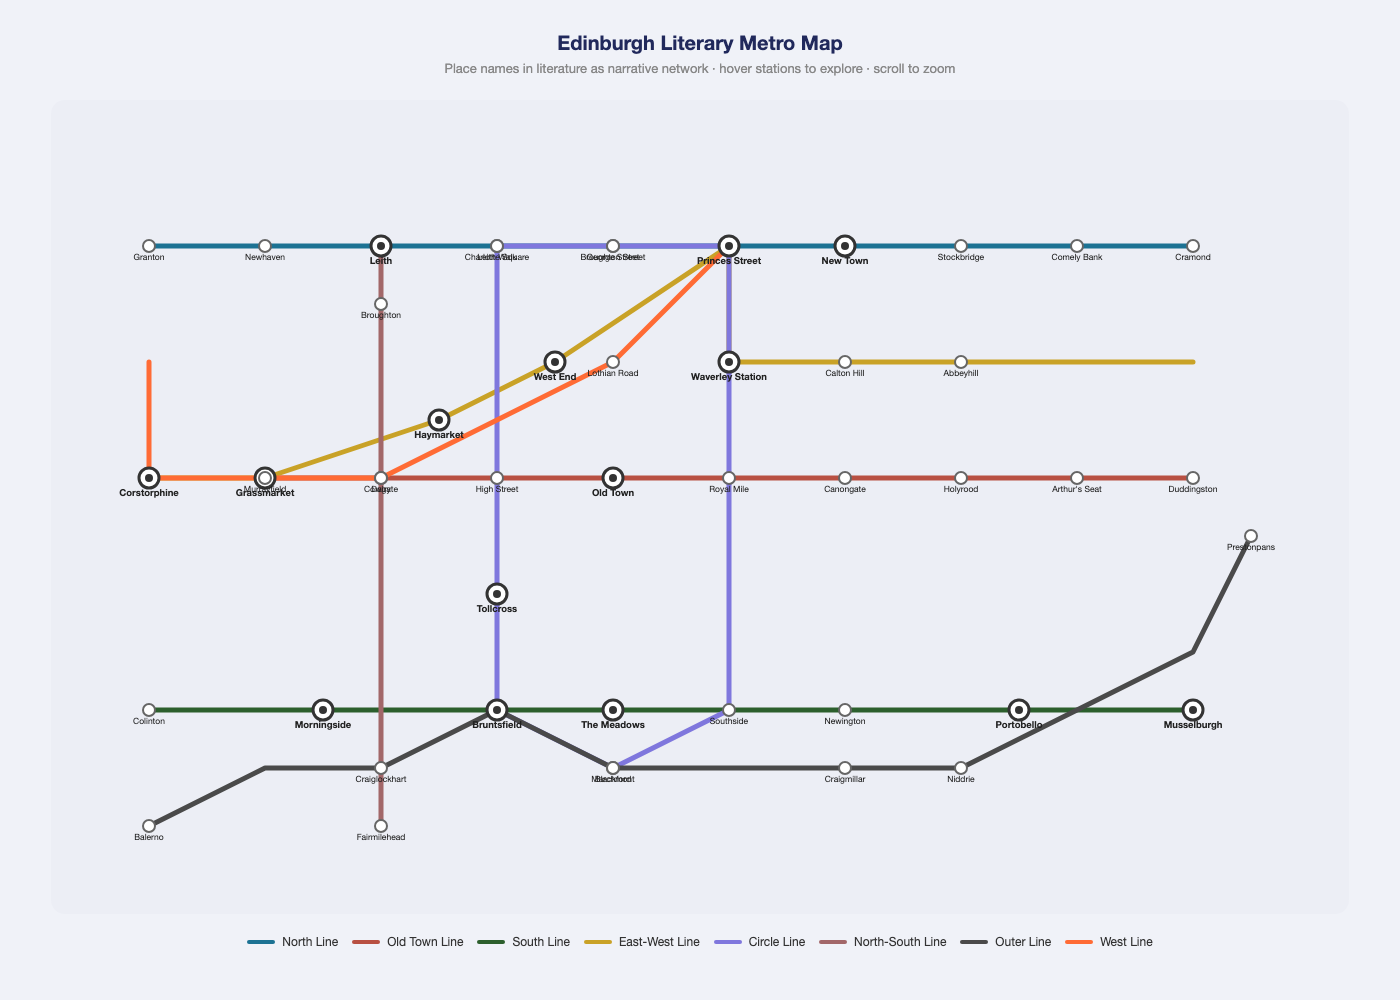
\includegraphics[width=0.55\textwidth]{figures/fig_metro_v1_geographic.png}
\caption{The initial hand-drawn metro-map prototype, before the redesign described in Section~\ref{sec:metro-redesign}. Lines follow geographic and cultural axes (a North Line, an Old Town Line, an East-West Line) chosen by inspection, with only 22\% of adjacent station pairs backed by measured co-occurrence, against 88\% for the redesigned map (Figure~\ref{fig:metro-after}).}
\label{fig:metro-before}
\end{figure}

Table~\ref{tab:metro-lines} lists the five lines produced by the community-detection pipeline described in Section~\ref{sec:metro-redesign}, with the number of home stations (stations whose narrative cluster this line is), the total station count including spliced-in interchange stops, total mentions summed across home stations, and the adjacency-backed diagnostic (the number of home-station-adjacent pairs, out of the total possible, that share at least one book in common).

\begin{table}[h]
\centering
\caption{The five metro-map lines and their composition.}
\label{tab:metro-lines}
\small
\begin{tabular}{lrrrl}
\toprule
Line & Home stations & Total stops & Mentions & Adjacency backed \\
\midrule
Smith's Edinburgh & 15 & 16 & 2{,}786 & 13/14 (93\%) \\
Leith \& Forth Corridor & 12 & 23 & 1{,}564 & 9/11 (82\%) \\
Scott's Edinburgh & 13 & 14 & 826 & 9/12 (75\%) \\
Welsh's Edinburgh & 12 & 12 & 494 & 11/11 (100\%) \\
Lockhart's Edinburgh & 5 & 5 & 202 & 4/4 (100\%) \\
\midrule
Total & 57 & --- & 5{,}872 & 46/52 (88\%) \\
\bottomrule
\end{tabular}
\end{table}

\noindent\small\textit{Note: ``Total stops'' exceeds ``home stations'' where a line has been joined by an interchange station whose home cluster is a different line (12 stations are interchanges across the whole map). The 22\% adjacency-backed figure for the earlier, hand-drawn eight-line version was computed over 67 same-line adjacent pairs, 15 of which shared a book.}

\section{Scale Exploration Summary}
\label{app:scale}

All six designs were re-tested at four benchmark author counts (2, 5, 20, and either 408 or the largest value practical for the design in question), plus a 2--3 book test for network and linear, using scale-exploration tools kept separate from the six canonical five-author prototypes (\texttt{data/processed/scale\_exploration/}). Table~\ref{tab:scale-summary} summarises the failure mode identified for each design; the full quantitative detail (per-$N$ tables, timing measurements, and the reasoning behind every scope choice) is recorded in the accompanying scale-exploration records submitted alongside this dissertation, rather than reproduced in full here.

\begin{table}[h]
\centering
\caption{Scaling failure mode identified for each of the six designs.}
\label{tab:scale-summary}
\small
\begin{tabular}{lp{3.2cm}p{6.8cm}}
\toprule
Design & Failure mode & Key evidence \\
\midrule
Radar & Visual overlap & Polygons indistinguishable by $N{=}20$; unreadable at 408; hover-to-isolate recovers single-author legibility at any $N$. \\
Bar-code & Navigation cost & 408 rows render in 20ms (no rendering problem) but the page is $\approx$45,000px tall, about 50 screens of scrolling. \\
Network & Visual overlap (graceful) & Core becomes a dense mass at 408 authors; periphery stays legible. Density is U-shaped in $N$ (79.6\% at 2 authors, $\approx$25\% at 5, 16.5\% at 408), driven by vocabulary non-overlap (Finding 1), not raw node count. \\
Linear & Horizontal sprawl & Canvas width grows from 1{,}100px (5 authors) to 29{,}790px (408 authors); a screenshot of the scrolled viewport looks unchanged because the same high-mention places sort leftmost regardless of $N$. \\
Small multiples & Computational cost (the only one) & Live Leaflet map initialisation degrades 3.6$\times$ per-panel from 50 to 408 authors (1.47s total at 408, measured directly); the one design where scale risks a real freeze, not just illegibility. \\
Metro & Clustering algorithm breakdown & Adjacency-backed proportion falls monotonically (96\%$\to$72\%, $N{=}2$ to 50); at $N{=}50$ one community reaches 75 stations because modularity detection judges it unsplittable despite exceeding the 18-station cap. \\
\bottomrule
\end{tabular}
\end{table}

\end{document}